
\chapter{Implementation}\label{implementation}

\section{Implementation Platform}\label{implementation-platform}

The validity and performance of the concept is put to test with a proof
of concept implementation. The reprojection method requires that the
radar position and velocity is known at all times. While there was no
precise source of ground truth data (like an IR ceiling camera system)
was easily available, the Kobuki robot platform provides a fairly good
odometry system and also allows to move the radar in a controlled way.

\subsection{Kobuki}\label{kobuki}

TODO

Good but not perfect odometry Ros Arm Limited performance Enough battery
capacity Omniradar FMCW Radar development kit

\includegraphics[width=0.5\textwidth]{https://rawgit.com/lalten/ma/master/models/kobuki.png}
Image source: \cite{DesignK2013}

\subsubsection{ROS integration}\label{ros-integration}

\subsubsection{Odroid}\label{odroid}

\subsection{Radar sensor}\label{radar-sensor}

\subsubsection{Devkit list}\label{devkit-list}

There are quite a few short-range UWB FMCW radar modules. The following
table compares some promising solutions.



\newlength{\colwidthA} \setlength{\colwidthA}{0.15\textwidth}
\newlength{\colwidthB} \setlength{\colwidthB}{0.2\textwidth}
\newlength{\colwidthC} \setlength{\colwidthC}{0.1\textwidth}
\newlength{\colwidthE} \setlength{\colwidthE}{0.10\textwidth}
\newlength{\colwidthF} \setlength{\colwidthF}{0.05\textwidth}
\newlength{\colwidthG} \setlength{\colwidthG}{0.15\textwidth}
\newlength{\maximheight} \setlength{\maximheight}{2cm}

{
\rowcolors{1}{ColorAlternatedRow}{}
\setlength\extrarowheight{4pt}
    
\begin{tabularx}{\linewidth}{%
  >{\setlength{\hsize}{.20\hsize}\raggedright\arraybackslash}X%
  >{\setlength{\hsize}{.25\hsize}}X%
  >{\setlength{\hsize}{.15\hsize}\raggedright\arraybackslash}X%
  >{\setlength{\hsize}{.15\hsize}\raggedright\arraybackslash}X%
  >{\setlength{\hsize}{.10\hsize}\raggedright\arraybackslash}X%
  >{\setlength{\hsize}{.20\hsize}\centering\arraybackslash}X%
}%
%\caption{Comparison of UWB radar development kits}\label{tab:devkits}

\hiderowcolors
\toprule
    Product &
    Note &
    $f_C$, $\Delta f$ &
    Antennas &
    DK Price &
    Picture \\
    \midrule
\endhead

\midrule
\multicolumn{6}{r}{Continued on next page} \\
\endfoot

\bottomrule
\endlastfoot
\showrowcolors

Omniradar RIC60A\footnote{\url{https://www.omniradar.com/products/}} &
High bandwidth. Presentation at SoC 2015\cite{Brouwer2015} &
60~GHz, 7~GHz &
On-chip, 1~Tx,~2~Rx &
\$4000 &
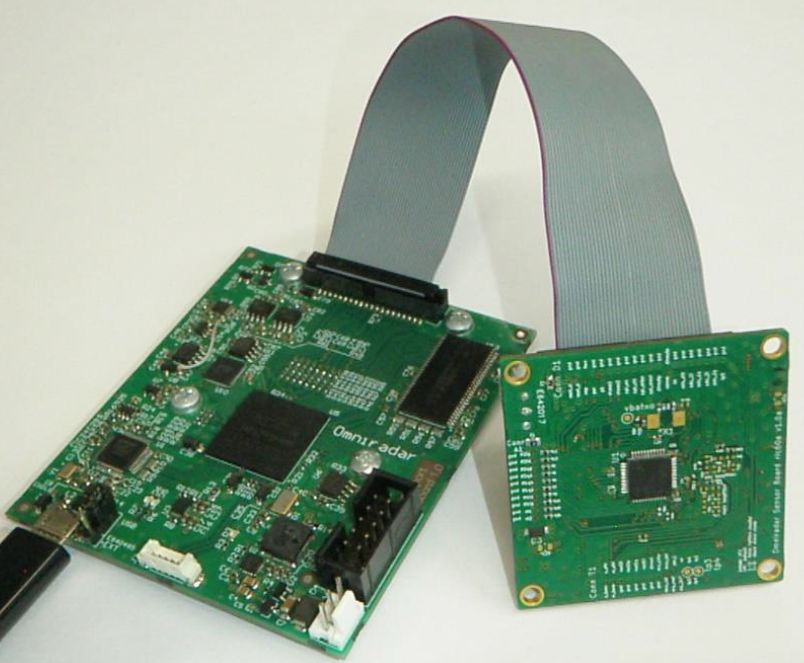
\includegraphics[max width=\hsize,max height=\maximheight,valign=t]{boards/img_omniradar.jpg}
\par\vspace{\extrarowheight}
\tabularnewline

Google / Infineon Soli\footnote{\url{https://www.infineon.com/cms/en/product/promopages/soli/}} &
Expected 2018. Sub-millimeter accuracy, running at over 10,000 frames per second \cite{Lien2016} &
60~GHz, 7~GHz &
In\nobreakdash-package, 2~Tx,~4~Rx &
? &
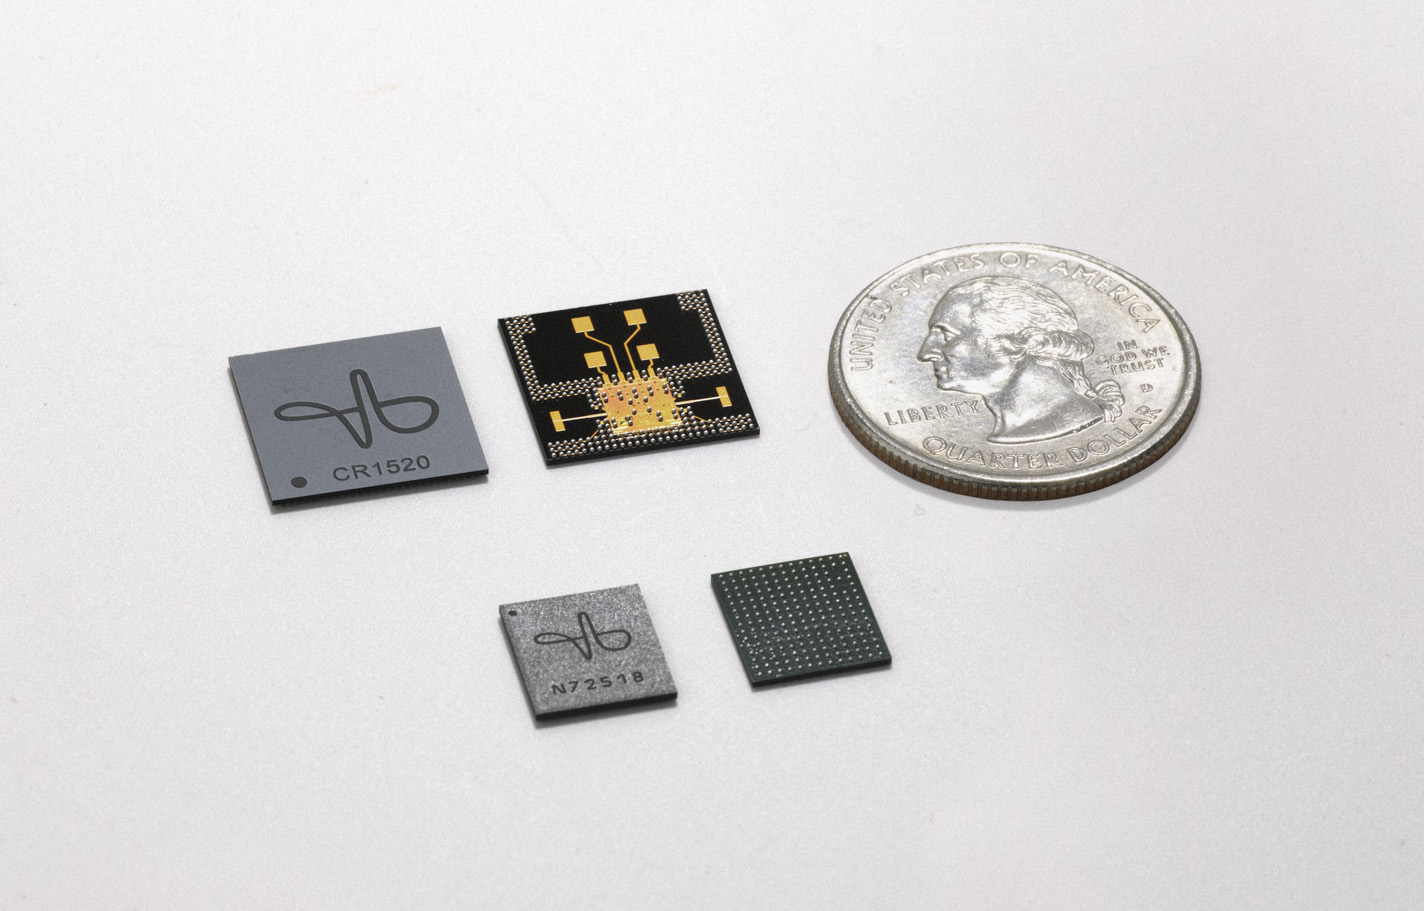
\includegraphics[max width=\hsize,max height=\maximheight,valign=t]{boards/img_soli.png}
\par\vspace{\extrarowheight}
\tabularnewline

Walabot Pro\footnote{\url{https://walabot.com/store/us/products/walabot-developer-pack.html}}&
3D configuration. Slow update rate&
6.8~GHz, 7~GHz &
On\nobreakdash-board, 9~Tx,~9~Rx&
\$599&
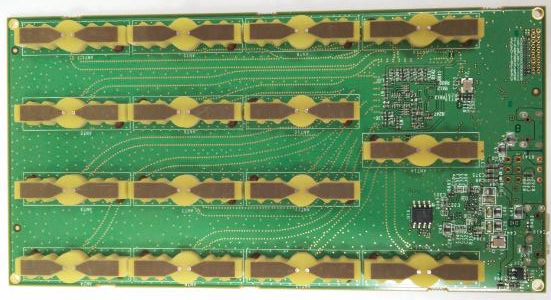
\includegraphics[max width=\hsize,max height=\maximheight,valign=t]{boards/img_walabot_1.png}
\par\vspace{\extrarowheight}
\tabularnewline

Bosch Prototype&
Prototype for In-wall pipe detection&
5.15~GHz, 6.7~GHz &
External, 2~Tx/Rx&
- &
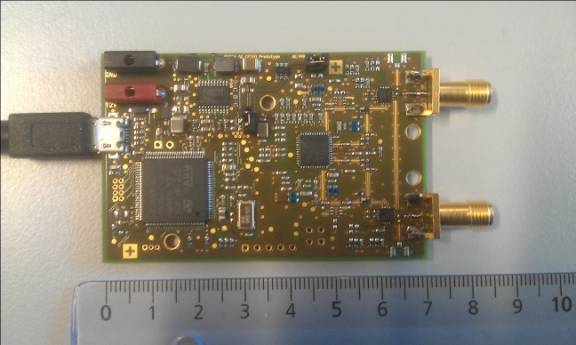
\includegraphics[max width=\hsize,max height=\maximheight,valign=t]{boards/img_bosch.jpg}
\par\vspace{\extrarowheight}
\tabularnewline

Silicon Radar SiRad Simple\footnote{\url{http://www.siliconradar.de/evalkits_e.html}}&
Has WiFi&
122~GHz, 6.4~GHz &
On-chip, 1~Tx,~1~Rx&
?&
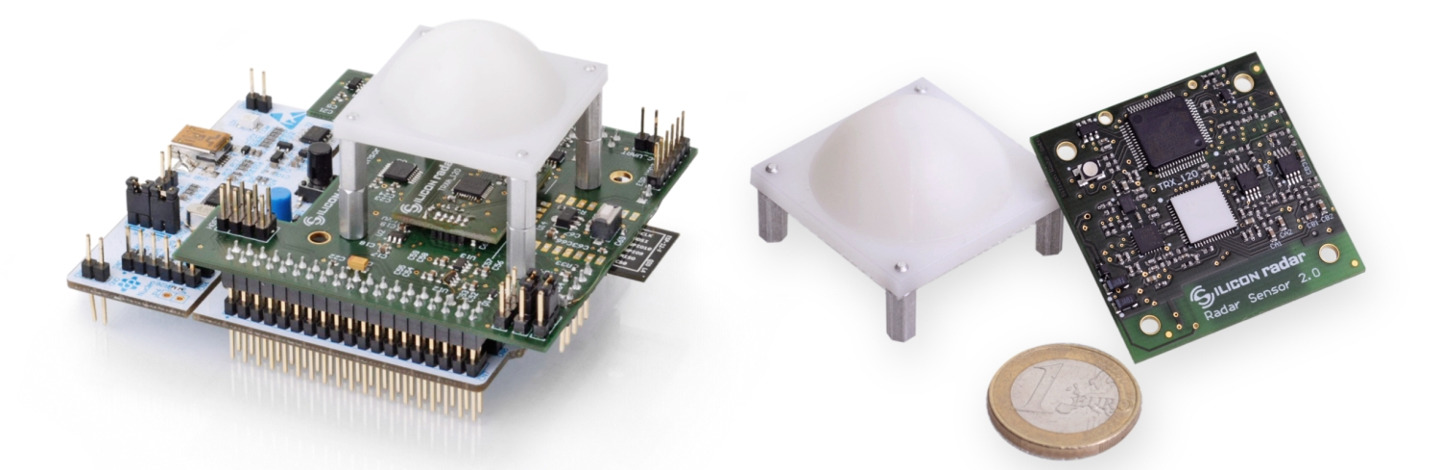
\includegraphics[max width=\hsize,max height=\maximheight,valign=t]{boards/img_silicon_radar.jpg}
\par\vspace{\extrarowheight}
\tabularnewline

Anokiwave AWMF-0117\footnote{\url{http://www.anokiwave.com/products/awmf-0117/index.html}}&
&
12.5~GHz, 4.5~GHz &
On-chip, 1~Tx/Rx&
?&
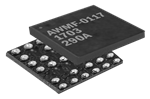
\includegraphics[max width=\hsize,max height=\maximheight,valign=t]{boards/img_anokiwave.png}
\par\vspace{\extrarowheight}
\tabularnewline

NXP Cocoon Radar\footnote{\url{Reuter2016}}&
Relatively small board. Presentation at FTF 2016\cite{Reuter2016}&
77~GHz, 4~GHz &
On\nobreakdash-board, 3~Tx,~4~Rx&
?&
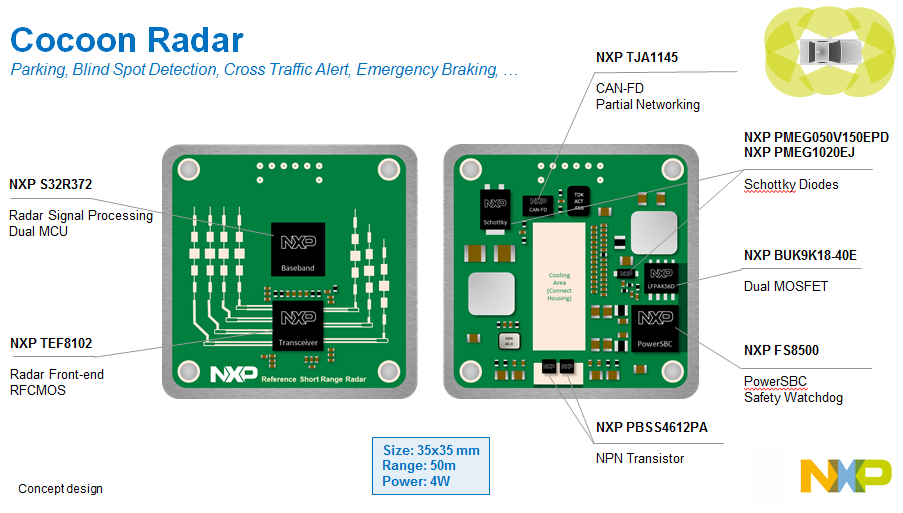
\includegraphics[max width=\hsize,max height=\maximheight,valign=t]{boards/img_cocoon.png}
\par\vspace{\extrarowheight}
\tabularnewline

TimeDomain P440\footnote{\url{http://www.timedomain.com/products/pulson-440/}}&
Can operate as multistatic radar or UWB communication node&
4~GHz, 1.7~GHz &
External, 2~Tx/Rx&
\$5000&
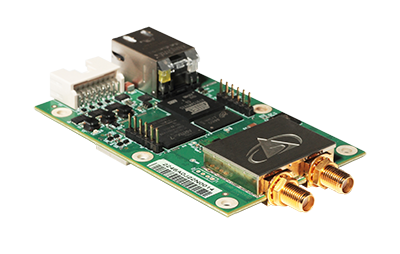
\includegraphics[max width=\hsize,max height=\maximheight,valign=t]{boards/img_p440.png}
\par\vspace{\extrarowheight}
\tabularnewline

Novelda Xethru X4M03\footnote{\url{https://www.xethru.com/xethru-development-platform.html}}&
&
8~GHz, 1.5~GHz &
On\nobreakdash-board, 1~Tx/Rx&
\$399&
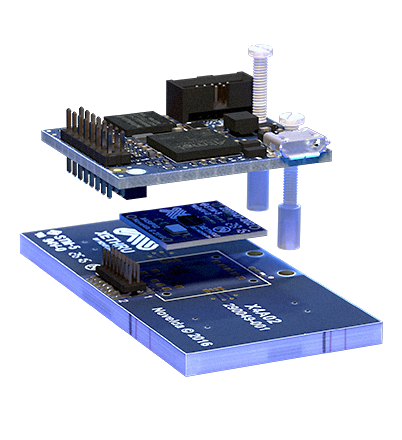
\includegraphics[max width=\hsize,max height=\maximheight,valign=t]{boards/img_xethru.png}
\par\vspace{\extrarowheight}
\tabularnewline

RFbeam MR2001\_RD\footnote{\url{https://www.rfbeam.ch/files/products/26/downloads/ProductBrief_MR2001_RD.pdf}}&
&
77~GHz, 1~GHz &
On\nobreakdash-board, 4~Tx,~6~Rx&
?&
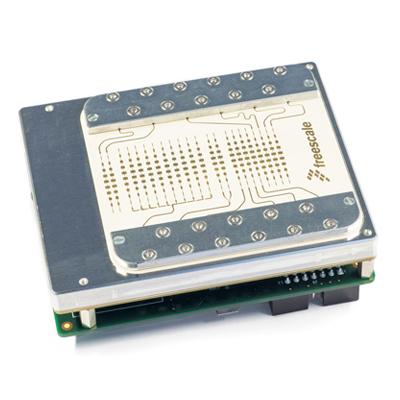
\includegraphics[max width=\hsize,max height=\maximheight,valign=t]{boards/img_rfbeam.jpg}
\par\vspace{\extrarowheight}
\tabularnewline

Inras 77Ghz Radarbook\footnote{\url{http://www.inras.at/en/products/radarbook.html}}&
Configurable FPGA processing chain&
77~GHz, 1~GHz &
On\nobreakdash-board, 4~Tx,~8~Rx&
\$7300&
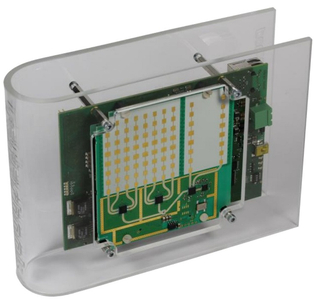
\includegraphics[max width=\hsize,max height=\maximheight,valign=t]{boards/img_radarbook.jpg}
\par\vspace{\extrarowheight}
\tabularnewline

Acconeer A1\footnote{\url{ http://www.acconeer.com/}}&
Sub-mm accuracy&
60~GHz, ? &
On-chip, ?&
?&
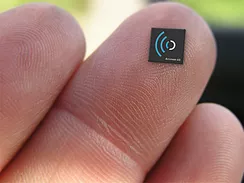
\includegraphics[max width=\hsize,max height=\maximheight,valign=t]{boards/img_acconeer.png}
\par\vspace{\extrarowheight}
\tabularnewline

Inras 24Ghz Radarbook\footnote{\url{dkradarbook}}&
&
24~GHz, 250~MHz &
On\nobreakdash-board, 4~Tx,~4~Rx&
\$7300&
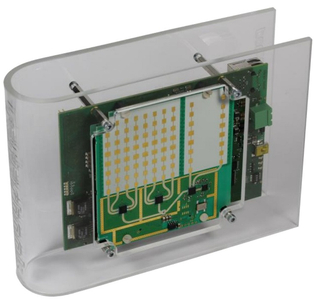
\includegraphics[max width=\hsize,max height=\maximheight,valign=t]{boards/img_radarbook.jpg}
\par\vspace{\extrarowheight}
\tabularnewline

Infineon BGT24-RFB2412-EVAL\footnote{\url{https://www.infineon.com/dgdl/?fileId=5546d46259d9a4bf0159f9f1fa503f1d}}&
&
24~GHz, 250~MHz &
On\nobreakdash-board, 1~Tx,~2~Rx&
\$1333&
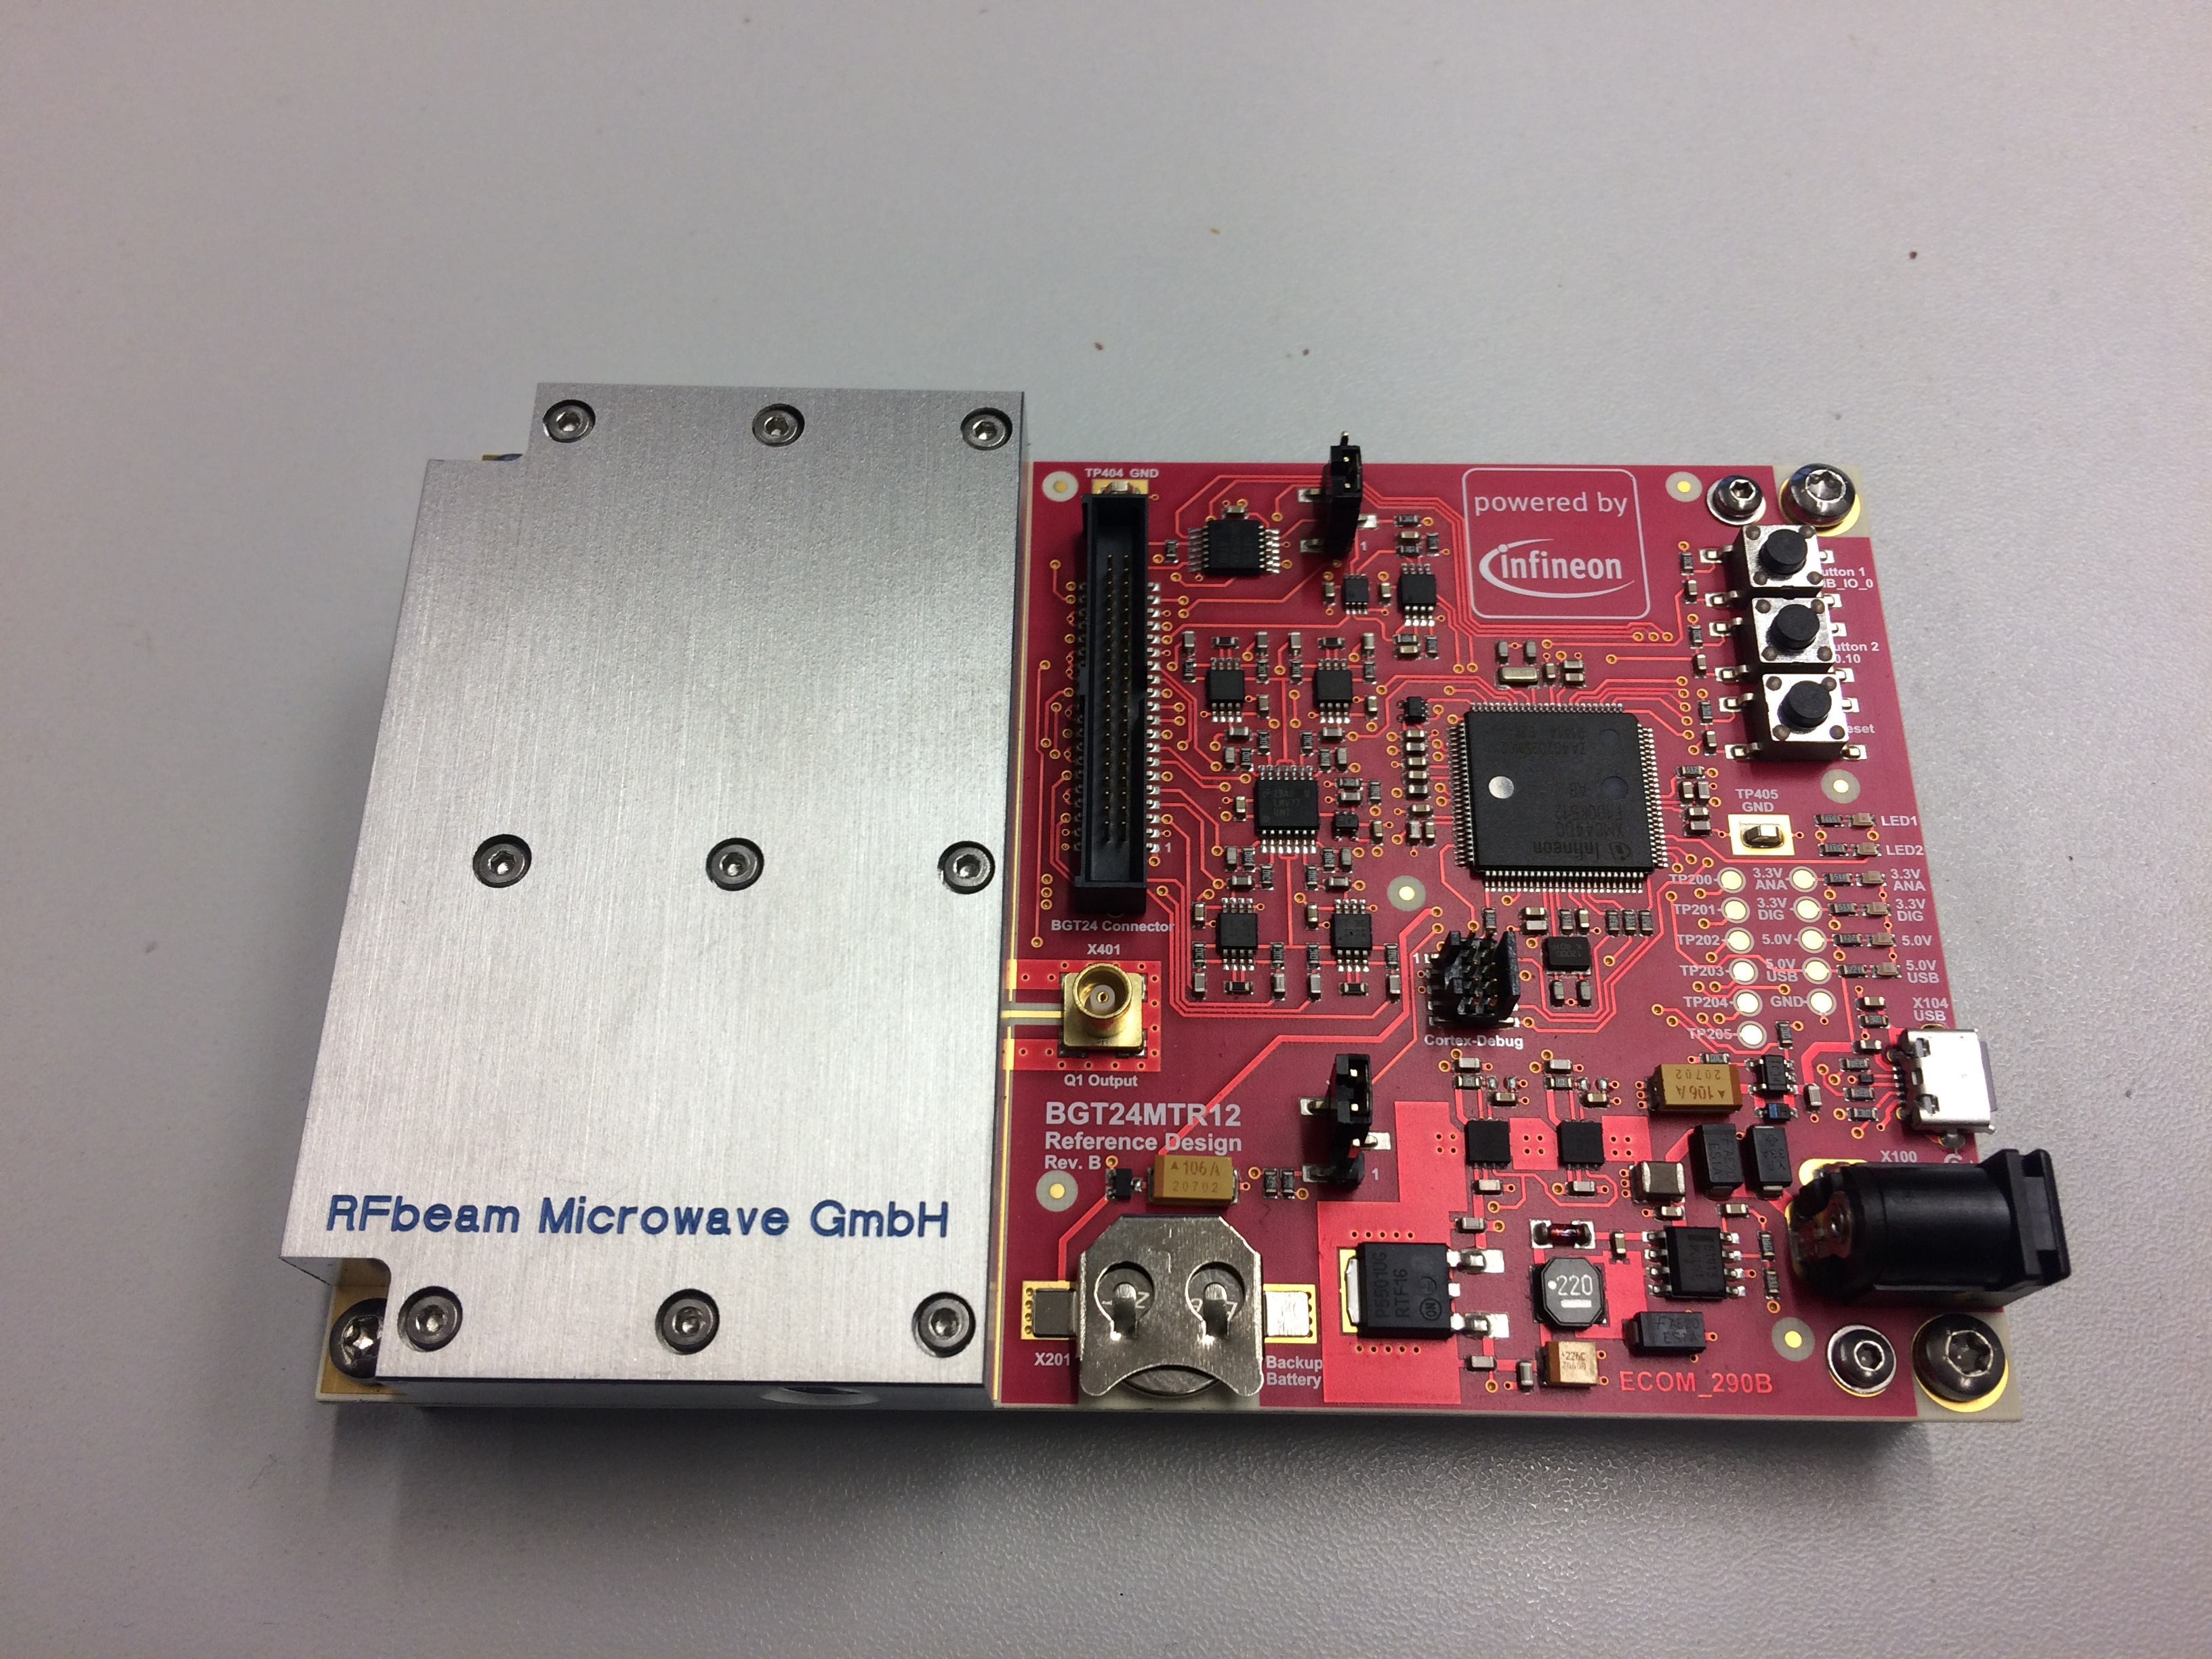
\includegraphics[max width=\hsize,max height=\maximheight,valign=t]{boards/img_bgt24.JPG}
\par\vspace{\extrarowheight}
\tabularnewline

IMST DK-sR-1200e\footnote{\url{http://webshop.imst.de/dk-sr-1200e-development-platform-for-24-ghz-fmcw-radar-application.html}}&
&
24~GHz, 250~MHz &
On\nobreakdash-board, 1~Tx,~2~Rx&
\$3333&
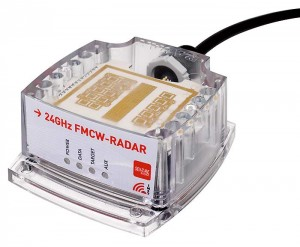
\includegraphics[max width=\hsize,max height=\maximheight,valign=t]{boards/img_IMST.jpg}
\par\vspace{\extrarowheight}
\tabularnewline

InnoSenT IVS-565\footnote{\url{http://www.innosent.de/fileadmin/media/dokumente/DATASHEETS_2016/Datenblatt_IVS-565.pdf}}&
&
24~GHz, 250~MHz &
On\nobreakdash-board, 1~Tx,~2~Rx&
?&
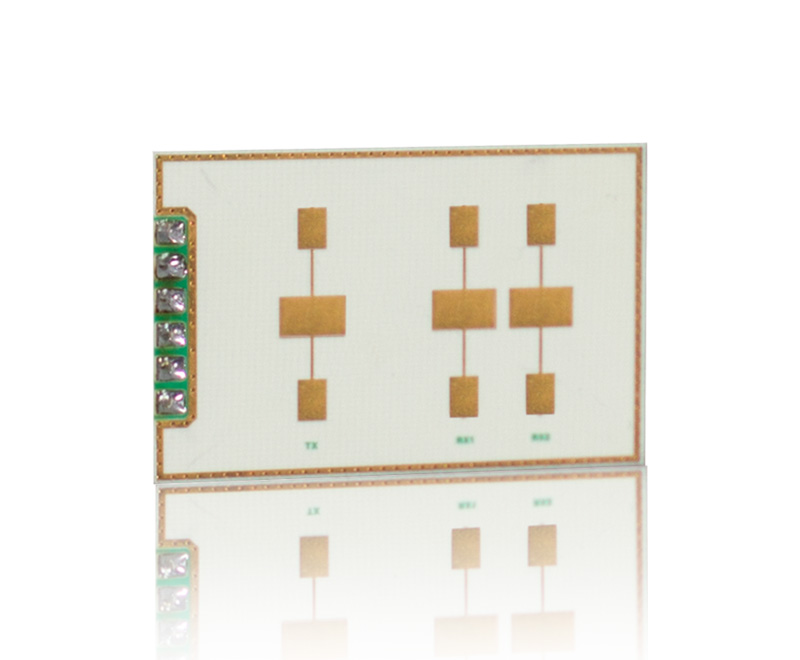
\includegraphics[max width=\hsize,max height=\maximheight,valign=t]{boards/img_innosent.jpg}
\par\vspace{\extrarowheight}
\tabularnewline

ST EVB-STradA431\footnote{\url{http://www.st.com/content/st_com/en/products/evaluation-tools/product-evaluation-tools/automotive-ic-eval-boards/evb-strada431.html}}&
SMA connectors for internal signals&
24~GHz, 250~MHz &
External, 1~Tx,~3~Rx&
?&
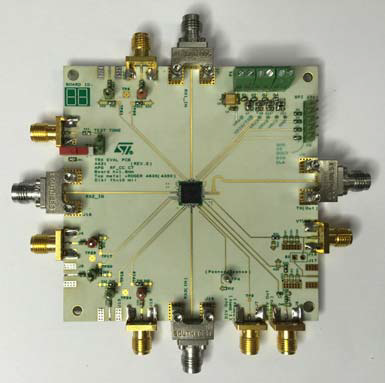
\includegraphics[max width=\hsize,max height=\maximheight,valign=t]{boards/img_ST.png}
\par\vspace{\extrarowheight}
\tabularnewline

OmniPreSense OPS241-A\footnote{\url{https://www.omnipresense.com/product/ops241-a/}}&
Arduino shield with BGT24LTR11&
24~GHz, 80~MHz &
On\nobreakdash-board, 1~Tx/Rx&
\$169&
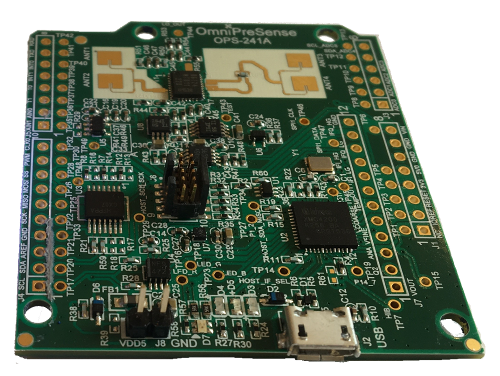
\includegraphics[max width=\hsize,max height=\maximheight,valign=t]{boards/img_omnipresense.png}
\par\vspace{\extrarowheight}
\tabularnewline

\bottomrule

\end{tabularx}

}


The most suitable modules are the ones with the highest bandwidth as
they give the highest resolution. Other beneficial properties are high
update rate, and higher number of antennas. A high degree of
configurability also helps during development. In the end, the Walabot
Pro, Omniradar RIC60A and a proprietary Bosch prototype were available
to be tested.

\subsubsection{Bosch Radar}\label{bosch-radar}

The Bosch radar presented some challenges under a Linux environment.
After its Matlab driver was patched for cross-platform compatibility, it
turned out that the on-board MCU's firmware had an incompatible protocol
format. A newer version of the prototype did work under Windows, but by
the time the board arrived, the decision to focus on Omniradar was made.

\subsubsection{Walabot}\label{walabot}

\href{https://www.vayyar.com/}{Vayyar} is an Israeli
\href{https://www.crunchbase.com/organization/vayyar}{startup} that was
founded in 2011. Coming from a medical background, they moved away from
use cases such as breast cancer detection towards general 3D imaging in
the consumer market with their Walabot sensor.

Vayyar's Walabot Pro sensor uses an 18-antenna MIMO array for 3D radar
imaging. Vayyar is very quiet about the technology and algorithms used
in their product and even the nature of the data that the sensor sends.
In their Python \href{https://api.walabot.com}{API documentation} they
showcase the modes of operation: 3d imaging, 2d imaging, object
tracking, pipe detection and raw data.

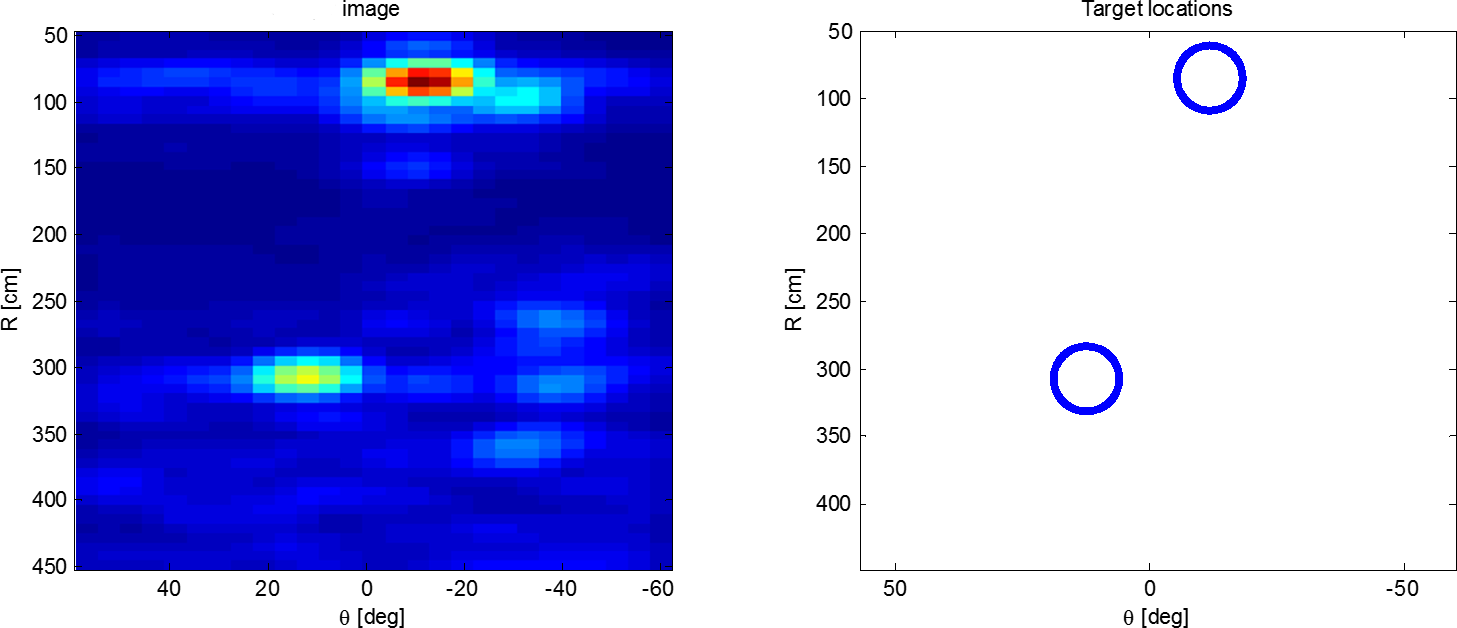
\includegraphics[width=0.5\textwidth]{https://rawgit.com/lalten/ma/master/figures/walabot_image.png}
Image source: https://api.walabot.com/\_features.html\#\_examples

The catch is however that it is almost impossible to do imaging without
background subtraction, which they do in all their examples. This works
well in scenarios where the sensor is at a fixed position or if the
region of interest is very small, like in the pipe detection scenario.
However, In the case of a robot-mounted sensor this does not work so
well.

At the time of writing, the only interesting published project is a fall
detection scenario \cite{Haider2017} by Haider, in which people can be
localized at intersections of vertically and horizontally oriented
heatmaps.

\subparagraph{Static range test}\label{static-range-test}

Figure \#REF shows the signal from two Walabot antenna pairs as it
records the scene in image \#REF with can stacks at \(0.5m\) \(1m\) and
\(1.5m\). The signal is very stable over time and shows next to no
noise. Unfortunately however it doesn't seem like the radar sensor can
detect the metal cans at all. The high frequency signal is the raw
signal as reported by the Walabot sensor. It is however hardly
believable that it was measured like this, as the visible base frequency
of the signal is around 7GHz. It was not possible to get any useful
information from Vayyar's technical support regarding this. The envelope
signal is a more interesting data source. It can easily be obtained from
the analytic signal, using \texttt{scipy.signal}'s Hilbert transform.
Another problem with the data is that the peaks of the envelope jitter
in range. This can be fixed by combination with another oddity: The last
180 samples rise very strongly in magnitude. If they are cut and
prepended to the first sample, they match up perfectly. Peaks can then
be detected in the signal (represented by the dots figure \#REF ) and
the range set to zero at the first peak. This eliminates the range
jitter completely. The reason is that the first peak is caused by
transmit antenna crosstalk and can thus be used as a timing reference
point.

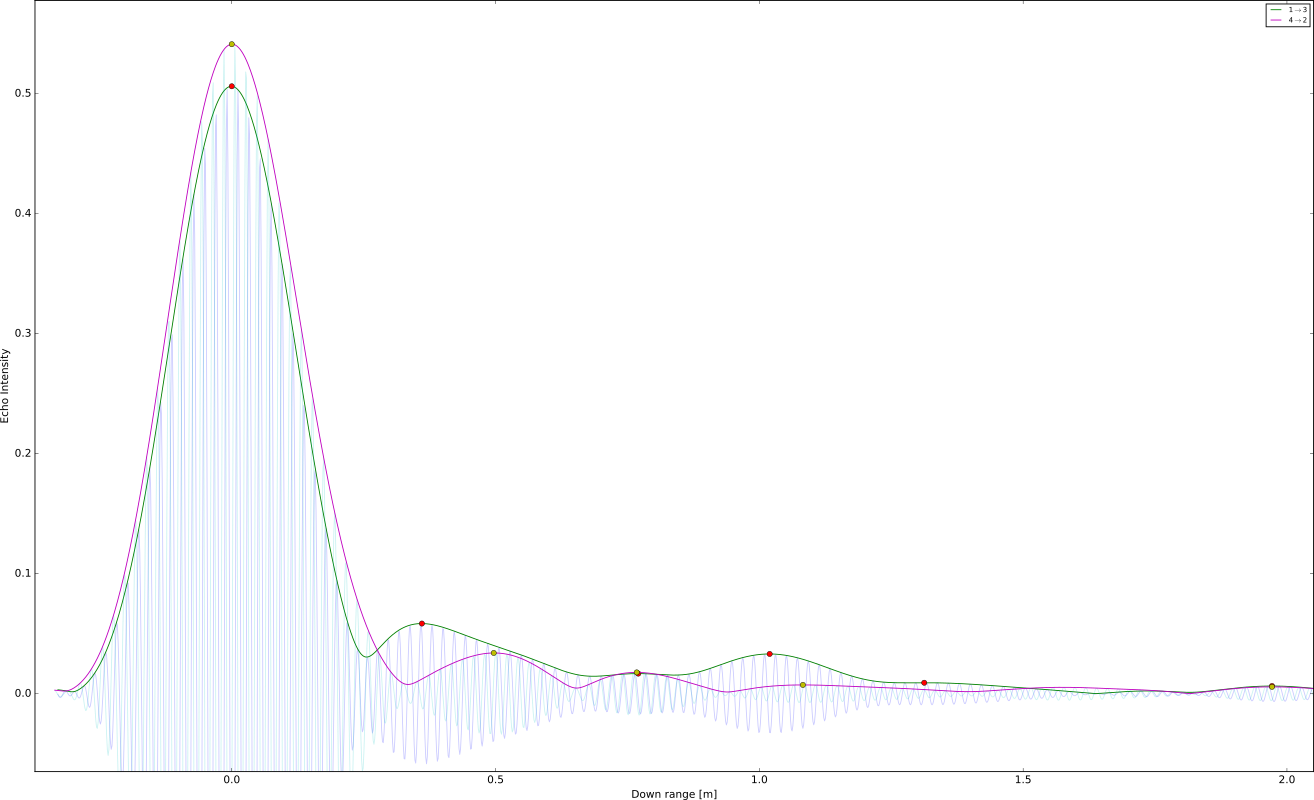
\includegraphics[width=0.5\textwidth]{https://rawgit.com/lalten/ma/master/figures/walabot_rangetest.png}
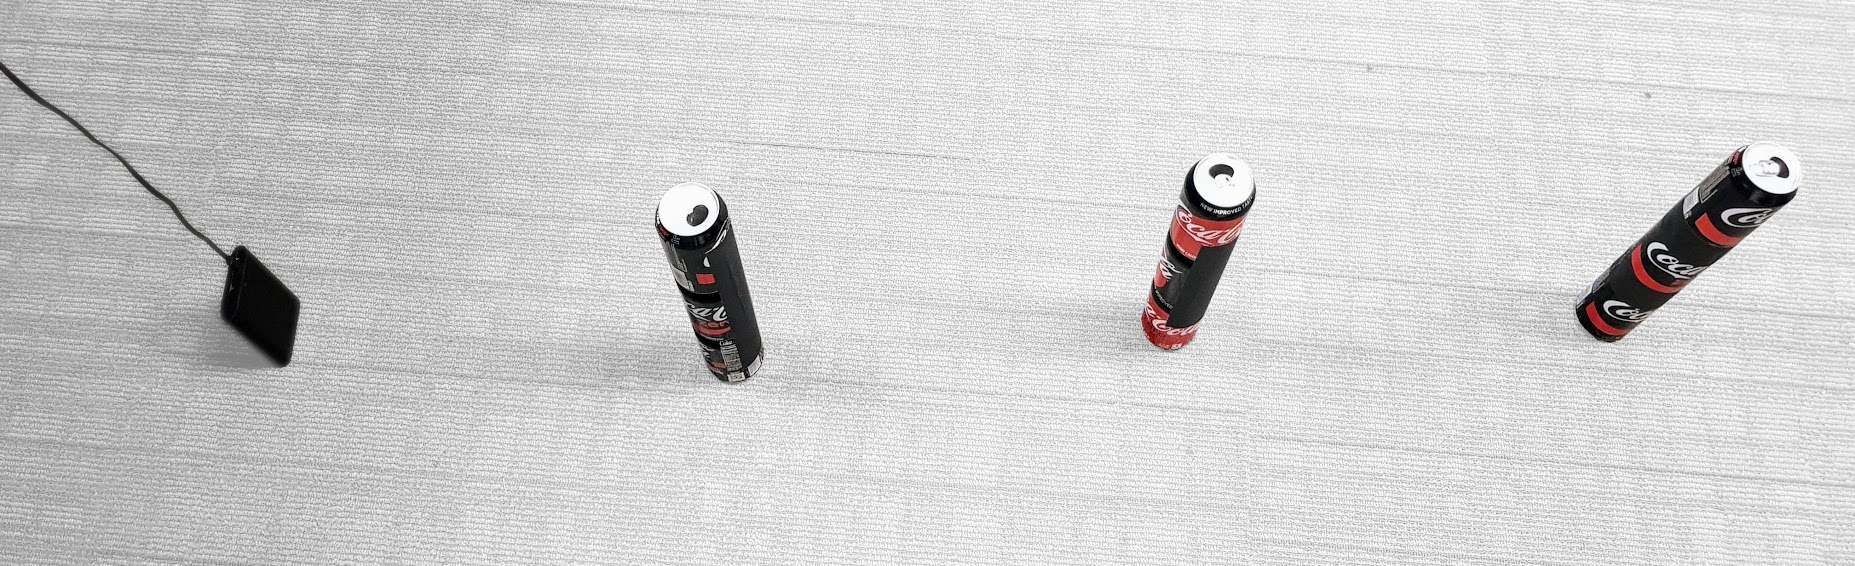
\includegraphics[width=0.5\textwidth]{https://rawgit.com/lalten/ma/master/pictures/experiment_walabot_rangetest.jpg}

\subparagraph{Dynamic range test}\label{dynamic-range-test}

Waving hands in front of the sensor did give a change in signal, but it
was difficult to interpret the data conclusively. To objectively test
the sensor's response, an aluminum plate that gave a strong echo signal
was taped to the Kobuki robot. The robot was then driven with a constant
speed away from the sensor and then towards the sensor as pictured in
\#REF.
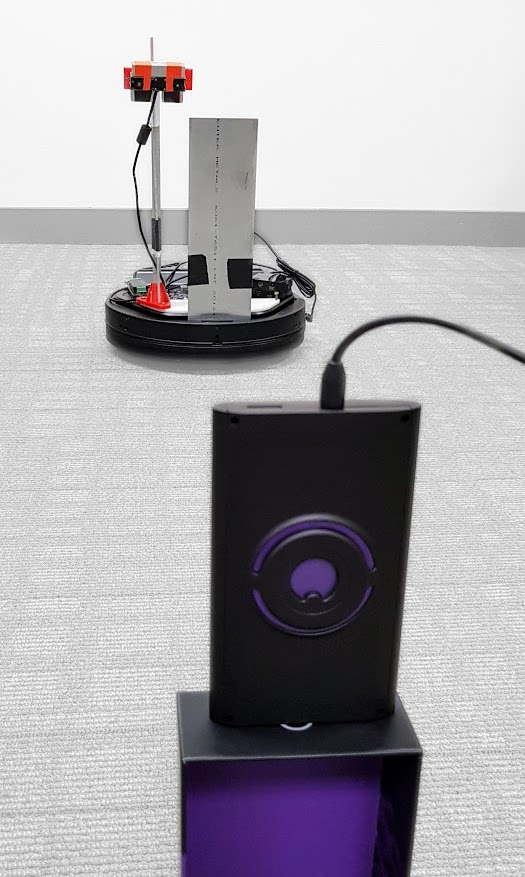
\includegraphics[width=0.5\textwidth]{https://rawgit.com/lalten/ma/master/pictures/experiment_walabot.jpg}

The sensor was sampled at a constant frequency in raw data mode. The
analytic signal of the range scans is stacked at the right end of the
matrix displayed in figure \#REF.

\begin{figure}
\centering
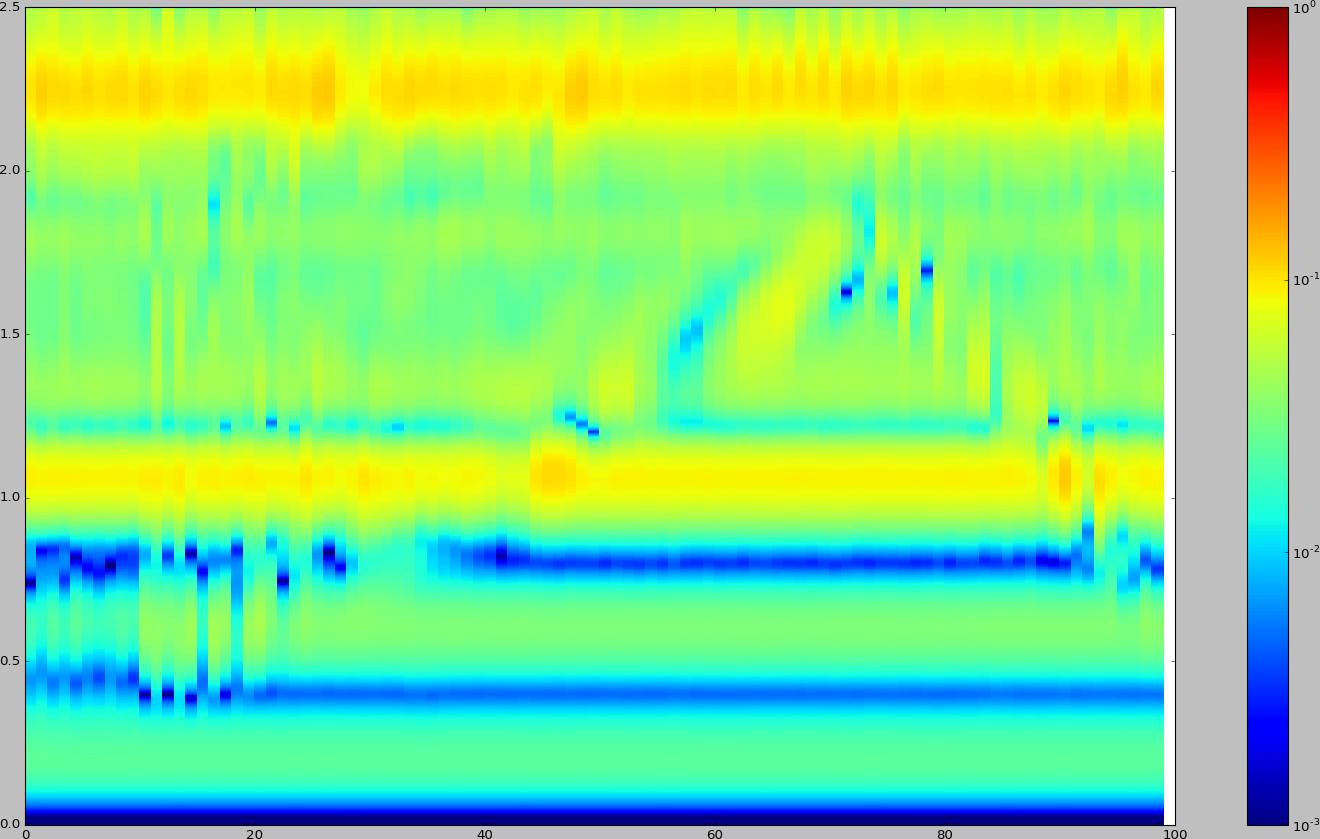
\includegraphics[width=0.5\textwidth]{https://rawgit.com/lalten/ma/master/figures/walabot_disttest.png}
\caption{restrict-height}
\end{figure}

The figure shows that the Walabot has problems with what looks like
standing waves. The great amount of background signal is also visible.
Because of its static nature, this can easily removed for a fixed radar.
As some Walabot reviewers have noticed \cite{Valens2016} this background
signal changes heavily and seemingly random when the sensor is moved.
This makes the signal processing very difficult.

Walabot advertises object detection capabilities. The catch with this
mode is however that the number of objects to be detected must be
configured first.

\section{Omniradar}\label{omniradar}

With its good range resolution and a good idea of its capabilities from
\cite{Ernst2016}, this sensor promised good results. As it was chosen as
a basis for the proof of concept implementation, it receives a more
detailed look.

Founded in 2010, \href{https://www.omniradar.com/}{Omniradar} is a Dutch
\href{https://www.crunchbase.com/organization/omniradar}{startup} that
claims to be the first to integrate a complete 60 GHz radar including
antennas and analog to digital conversion in one chip.

With the RIC60-A they offer a Radar Development Kit (RDK) that gives
7GHz of bandwidth on two receiving antennas. An Altera Cyclone IV FPGA
handles the signal acquisition and communication. Figure \#REF shows the
radar IC and how the three antennas are integrated in silicon.

%\includesvg[width=0.5\textwidth]{https://rawgit.com/lalten/ma/master/pictures/slide_RIC60A}
Source: \cite{Brouwer2015} p.9

The radar sensor's beam is fan shaped, which means it is fairly
sensitive over a wide angle in azimuth direction, but relatively focused
in elevation. This makes it a very good candidate for the radar
reprojection, as targets can be seen from the robot in a wide field of
view, but floor and ceiling reflections are kept at a minimum. Of course
the sensor can also be rotated. Omniradar also supplies a horn-like
extension for the sensor board, which forms the radar sensitivity into a
pencil-shaped beam that is very focused at a narrow field of view.

\begin{figure}
\centering
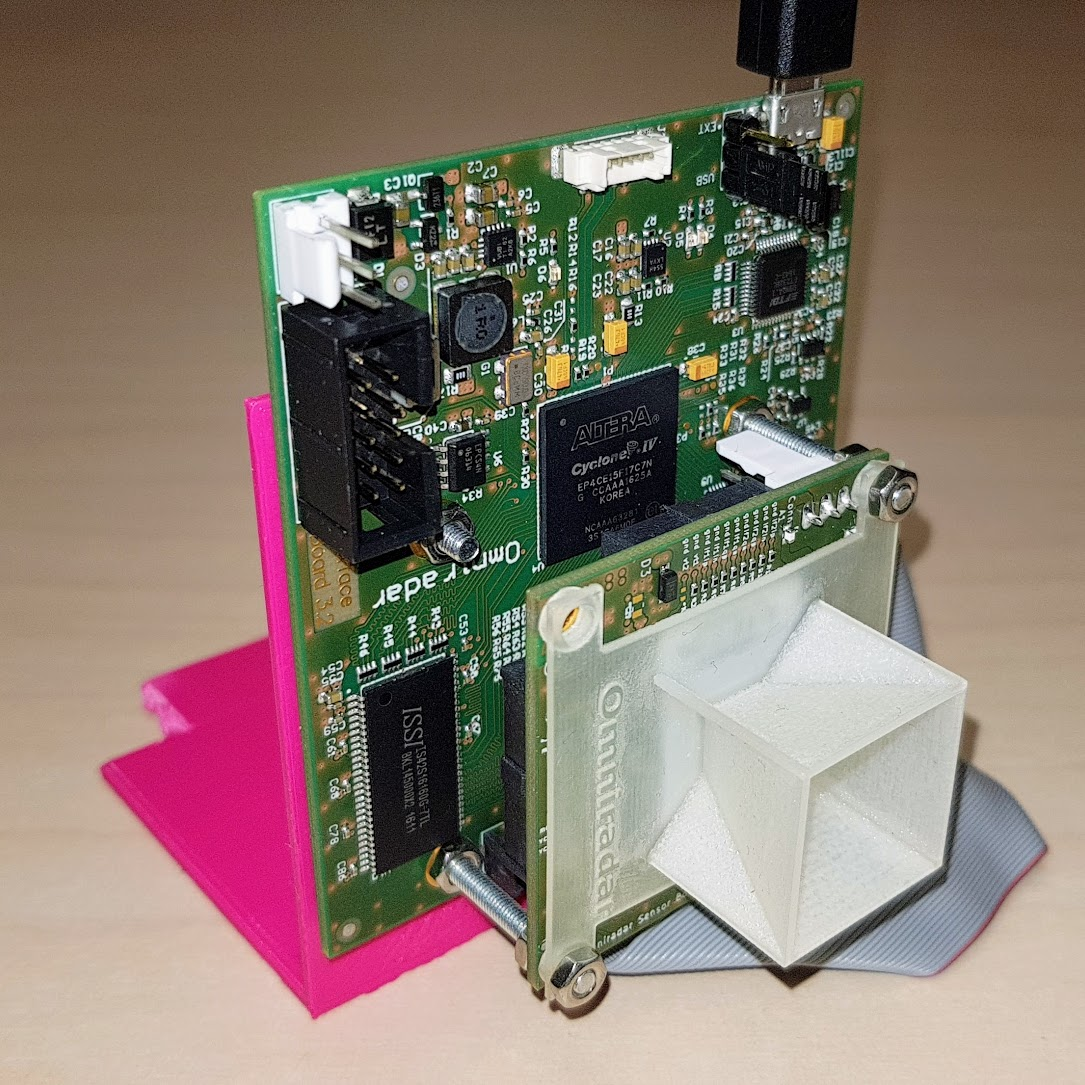
\includegraphics[width=0.5\textwidth]{https://rawgit.com/lalten/ma/master/pictures/omniradar.jpg}
\caption{restrict-height}
\end{figure}

\subsection{Radar mount}\label{radar-mount}

A 3D-printed part makes sure that the radar sensor is firmly mounted on
the robot as it explores its environment. The part was designed in
\href{http://www.openscad.org/}{OpenSCAD} and printed on a
\href{https://3dprinter.dremel.com/}{Dremel 3D printer}. The bottom
mount hole positions were extracted from the mechanical drawings of the
Kobuki Base \cite{YujinRobot2012}; the side holes from the Altium layer
document of the version 3.2 Omniradar interface board
\cite{Omniradar2014}.
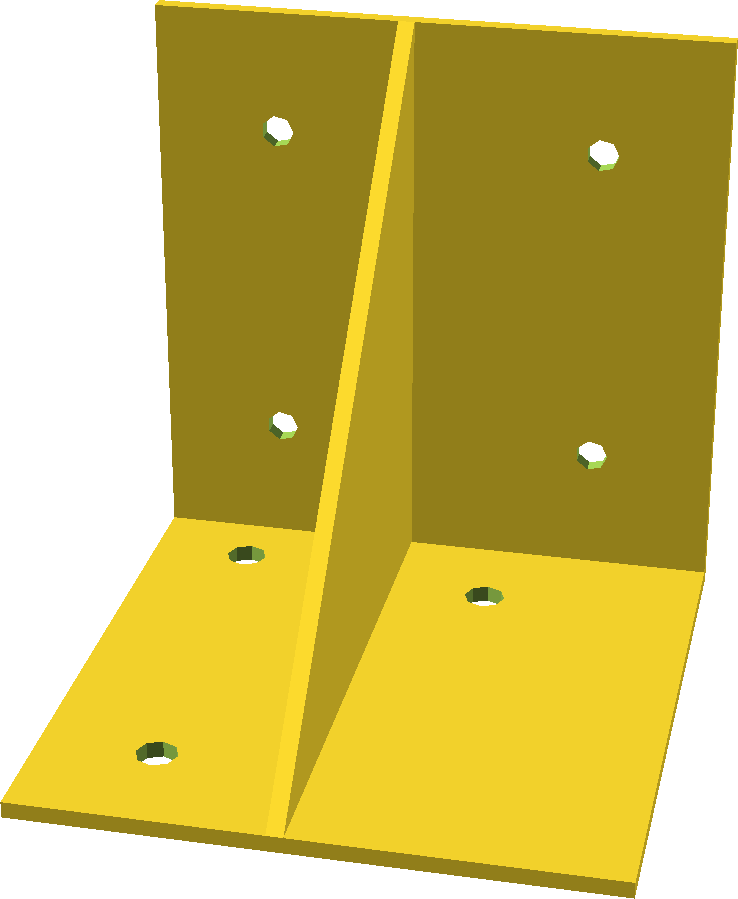
\includegraphics[width=0.5\textwidth]{https://rawgit.com/lalten/ma/master/models/mount.png}
When rotated to face to the left side of the robot, the RPLidar mount
was in the way, so parts of the print had to be clipped off.

Two screws hold the Omniradar interface board to the mount. The other
two mounting holes in the interface board hold the Omniradar sensor
board. The horn extension can be affixed to these screws as well. If a
different sensor orientation is necessary, the sensor board can be
rotated by 90 degrees, thanks to the symmetric layout.

\subsection{Doppler sensitivity}\label{doppler-sensitivity}

The Omniradar FMCW radar is not sensitive enough to use the Doppler
speed directly. The following example illustrates this.

The RIC60A has a sensitivity of \(400 \frac{Hz}{m/s}\). A target with a
doppler speed of \(0.02 m/s\) (A low speed at which the Kobuki robot
still moves continuously and without jerking) will cause a frequency
spike with a shift of \(8Hz\) in the FMCW beat frequency.

The speed resolution capability is inversely proportional to the
measurement or acquisition time. A 10 ms long acquisition gives a 100 Hz
frequency resolution, or a speed resolution of 0.9 km/h (or 0.25 m/s).

Sampling frequency \(F_s=25MHz\) and RIC60A Doppler sensitivity,
\(S_D = 400 \frac{Hz}{m/s}\) are constant values of the Omniradar RDK.

Given a chirp duration of \(T_{chirp} = 2.5ms\), we get
\(N_s = t_{chirp} F_s = 62500\) Samples,
\(N_r = \lfloor \frac{N_s}{2} \rfloor = 31250\) Samples per
up/downsweep, \(dF = \frac{F_s}{N_r - 1} = 800 Hz\) FFT frequency bin
width and hence a Doppler resolution of \(\frac{dF}{S_D} = 2 m/s\).

Even with subsample peak interpolation the accuracy will not be very
good and targets will be reprojected at imprecise angles.

It would be possible to use higher precision equipment. But another
solution is to track the movement of target peaks in the range profile,
using the Peak Gradient algorithm.

\subsection{Optimal chirp time
configuration}\label{optimal-chirp-time-configuration}

The chirp duration \(t_{chirp}\) is configurable and has an effect on
how the raw range profile data will look like.

\textbf{Very short durations} (\(<2ms\)) incur a considerable processing
overhead to acquisition time ratio and have a very low SNR.
\textbf{Short durations} (\(<5ms\)) have acceptable SNR, and are more
efficient with respect to overhead. \textbf{Long durations} (\(>15ms\))
have good SNR, and don't create a lot of overhead. However at higher
robot speeds, target peaks get blurred over several range bins as they
move in range. Less intense target echos are more difficult to detect
then. \textbf{Very long durations} (\(>20ms\)) required the Omniradar
driver to be patched on Linux so as not to freeze when chirps longer
than \(20ms\) are requested. Even with the patched driver the RDK's FPGA
firmware is not very reliable at sending large volumes of data at once
and corrupts packet headers or aborts transmissions intermittently.

The optimal range was empirically found to lie between \(2ms\) and
\(10ms\).

Figure \#REF shows the chirp efficiency
\(\eta = \frac{n_{chirp}~t_{chirp}}{t_{msg}}\), with number of
consecutive sweeps \(n_{chirp}\) (two in the graph's data source), chirp
length \(t_{chirp}\), and \(t_{msg}\) the time since last radar message.

\begin{figure}
\centering
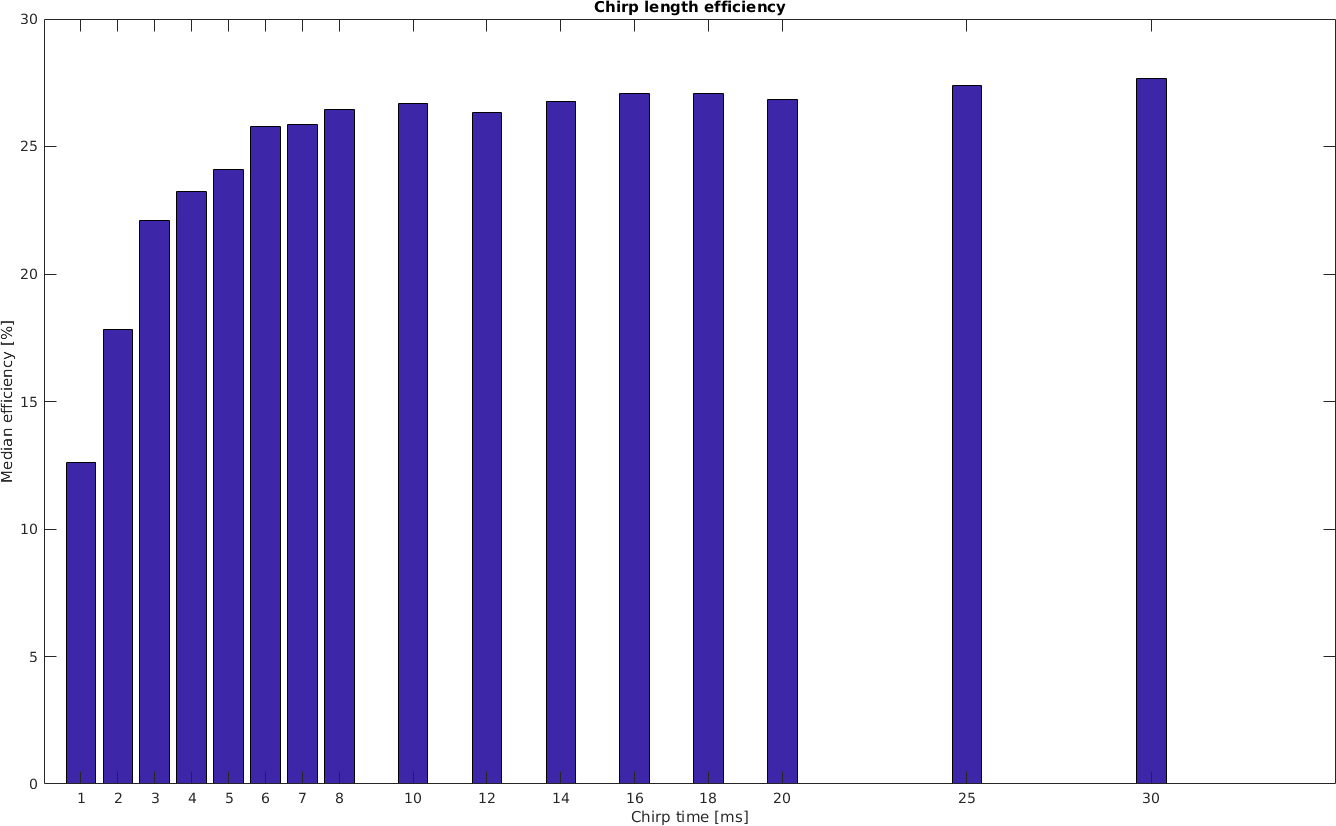
\includegraphics[width=0.5\textwidth]{https://rawgit.com/lalten/ma/master/figures/fig_chirp_eff.png}
\caption{restrict-height}
\end{figure}

The chirp length has an effect on accuracy and resolution. Figure \#REF
shows how short chirp times

\begin{figure}
\centering
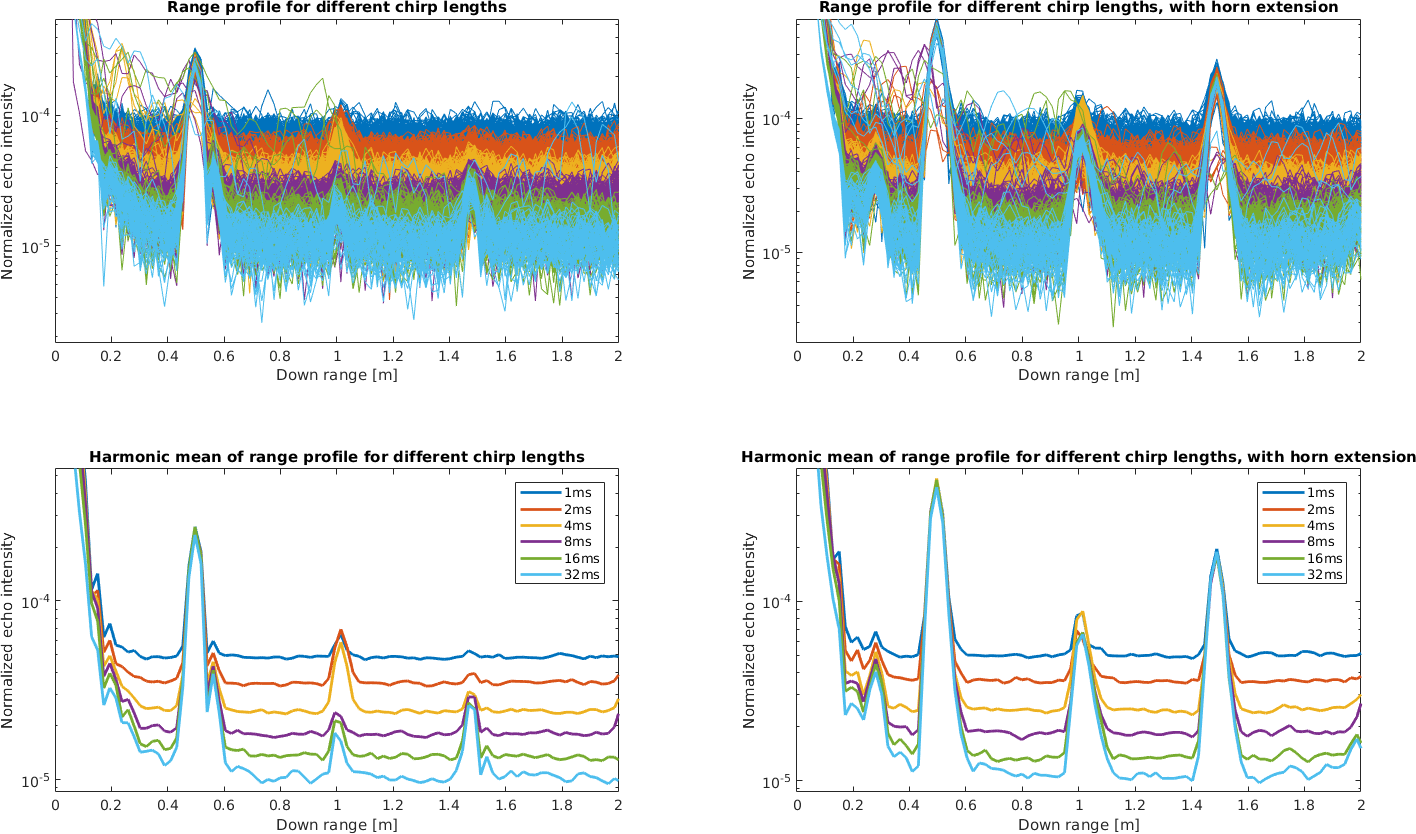
\includegraphics[width=0.5\textwidth]{https://rawgit.com/lalten/ma/master/figures/fig_compare_chirp_times.png}
\caption{restrict-height}
\end{figure}



\section{Omniradar ROS driver}\label{omniradar-ros-driver}

The Omniradar RIC60A comes with a precompiled Matlab MEX driver library.
This works well in a Windows OS on x86-based computers with a Matlab
installation. An early goal was to have the robot carry the radar module
around wireless. One option would have been to mount a Windows laptop on
the Kobuki. However, Omniradar was kind enough to provide the author
with the driver sources under an NDA agreement. This allowed recompiling
the MEX driver for Linux systems. There were some issues with FTDI's
D2XX serial communication library that had to be fixed for Linux
systems. One challenge with the D2XX driver was that Ubuntu
automatically loads the regular FTDI serial IO driver,
\texttt{ftdi\_sio}. This could be solved by unbinding the driver in a
set of udev rules
\href{https://stackoverflow.com/questions/44529376}{{[}ref{]}}. Another
issue was that due to a bug in the D2XX implementation, the Omniradar
driver would freeze when more than 2MB of data (equivalent to a 20ms
FMCW chirp) were requested. After a lot of debugging, this could be
solved by never requesting a bigger amount of data than was already
available in the D2XX buffer.

\subsection{C++ bindings and library}\label{c-bindings-and-library}

Since Matlab does not run on Arm arch processors such as the Odroid on
the Kobuki robot, a new set of platform-independent C++ bindings was
added to the driver. The C++ bindings serve the same purpose as the
Matlab bindings.

To include the library, some files need to be installed or pointed to by
the binary that needs to use it.

\begin{longtable}[]{@{}lll@{}}
\toprule
\begin{minipage}[b]{0.06\columnwidth}\raggedright\strut
File\strut
\end{minipage} & \begin{minipage}[b]{0.15\columnwidth}\raggedright\strut
Default install destination\strut
\end{minipage} & \begin{minipage}[b]{0.10\columnwidth}\raggedright\strut
Purpose\strut
\end{minipage}\tabularnewline
\midrule
\endhead
\begin{minipage}[t]{0.06\columnwidth}\raggedright\strut
omniradar.h\strut
\end{minipage} & \begin{minipage}[t]{0.15\columnwidth}\raggedright\strut
/usr/local/include\strut
\end{minipage} & \begin{minipage}[t]{0.10\columnwidth}\raggedright\strut
Library header file\strut
\end{minipage}\tabularnewline
\begin{minipage}[t]{0.06\columnwidth}\raggedright\strut
libomniradar.so\strut
\end{minipage} & \begin{minipage}[t]{0.15\columnwidth}\raggedright\strut
/usr/local/lib\strut
\end{minipage} & \begin{minipage}[t]{0.10\columnwidth}\raggedright\strut
dynamically linked shared object\strut
\end{minipage}\tabularnewline
\begin{minipage}[t]{0.06\columnwidth}\raggedright\strut
51-omniradar.rules, 52-omniradar.rules\strut
\end{minipage} & \begin{minipage}[t]{0.15\columnwidth}\raggedright\strut
/etc/udev/rules.d/\strut
\end{minipage} & \begin{minipage}[t]{0.10\columnwidth}\raggedright\strut
Udev rules to unbind ftdi\_sio\strut
\end{minipage}\tabularnewline
\bottomrule
\end{longtable}

If the driver source is available, installing the files can be
accomplished from the source directory with

\begin{Shaded}
\begin{Highlighting}[]
\FunctionTok{mkdir}\NormalTok{ build }\KeywordTok{\&\&} \BuiltInTok{cd}\NormalTok{ build}
\FunctionTok{cmake}\NormalTok{ -DCPP_BINDINGS=ON -DMATLAB_BINDINGS=OFF ..}
\FunctionTok{make}
\FunctionTok{sudo}\NormalTok{ make install}
\end{Highlighting}
\end{Shaded}

The driver can then be included in an application. Note that since it is
dynamically linked, the \texttt{ftd2xx}, \texttt{pthread} and
\texttt{dl} libraries dependencies also need to be linked. In a Catkin
\footnote{Catkin is the CMake-based ROS build system} CMakeLists.txt
this would look like

\begin{Shaded}
\begin{Highlighting}[]
\KeywordTok{target_link_libraries}\NormalTok{(}
  \VariableTok{\$\{PROJECT_NAME\}}\NormalTok{_node}
\NormalTok{  omniradar}
\NormalTok{  ftd2xx}
\NormalTok{  pthread}
\NormalTok{  dl}
  \VariableTok{\$\{catkin_LIBRARIES\}}
\NormalTok{)}
\end{Highlighting}
\end{Shaded}

The C++ library offers the same functions as Omniradar's Matlab driver,
with two differences. The optional device index number is 0-based
instead of 1-based and the AquireEcho functions return (a shared pointer
to) packed data instead of unpacked data for performance reasons. With
the

\begin{Shaded}
\begin{Highlighting}[]
\AttributeTok{static} \BuiltInTok{std::}\NormalTok{shared_ptr< }\BuiltInTok{std::}\NormalTok{vector<}\BuiltInTok{std::}\NormalTok{vector<}\DataTypeTok{uint8_t}\NormalTok{> > > demultiplex(}\BuiltInTok{std::}\NormalTok{vector<}\DataTypeTok{uint32_t}\NormalTok{> \&packed_data);}
\end{Highlighting}
\end{Shaded}

function, the library offers an easy way to demultiplex the packed data
array into a (shared pointer to a) vector of four vectors - one for each
echo signal of the I/Q channel of left and right receiving antenna.

Useage is simple as the driver follows the RAII principle. Allocation of
an object of type \texttt{Omniradar} causes the library to fully
initialize the RIC60A RDK. After that, the configuration string and the
VCO tuning curve should be set. Omniradar provides some Matlab example
code that measures the sensor's VCO tuning curve. The easiest way to
bring this tuning curve into the C++ domain is to
print\footnote{`['A' 10 'B']` is a quick way to print a newline character between `A` and `B`}
it as C style array, e.g.~with

\begin{Shaded}
\begin{Highlighting}[]
\NormalTok{[}\StringTok{'#pragma once'} \FloatTok{10} \StringTok{'std::vector<double>'} \FloatTok{10} \StringTok{'vco_tune \{'}\NormalTok{, sprintf(}\StringTok{'\%.100g, '}\NormalTok{, VCOtune), }\StringTok{'\};'}\NormalTok{]}
\end{Highlighting}
\end{Shaded}

and then saving the resulting string as \texttt{vco\_tune.h} include
file.

This setup allowed the development of a ROS node that handles
communication with the radar module on the Linux/Arm based Kobuki robot.

\subsection{ROS node}\label{ros-node}

A new \texttt{omniradar} ROS package was developed to support the use of
the Omniradar sensor within the ROS environment. A set of
\texttt{roslaunch} launchfiles comes with the package that support the
startup of the Kobuki robot in teleoperation mode, optionally together
with lidar-based Cartographer slam, AMCL localization and an Astra
Orbbec RGBD camera. A simple version to start the only the node to get
radar data would be:

\begin{verbatim}
<launch>
  <node pkg="omniradar" type="omniradar_node" name="omniradar_node" output="screen">
    <param name="n_sweeps" value="1" />
    <param name="t_sweep" value="5" />
  </node>
</launch>
\end{verbatim}

The node sends out the ROS topic \texttt{/omniradar\_node/radar\_raw} of
the custom \texttt{RadarEcho} type, which is defined in RadarEcho.msg as

\begin{verbatim}
Header header
string ric_config
uint8 n_sweeps
float64 t_sweep
uint32[] packed_echo
\end{verbatim}

Early versions of the driver unpacked the radar echo bitstream inside
the node and were able to use standard ROS message types like the
\texttt{std\_msgs/ByteMultiArray} message. However, sending out the
packed bitstream proved to be much more efficient in terms of chirp
efficiency \(\eta\). The custom message type also allows to send out the
configuration (RIC configuration string, number and length of FMCW
sweeps) that was used to attain the message's echo. The message's
timestamp and sequential ID is contained in the regular
\texttt{std\_msgs/Header}.
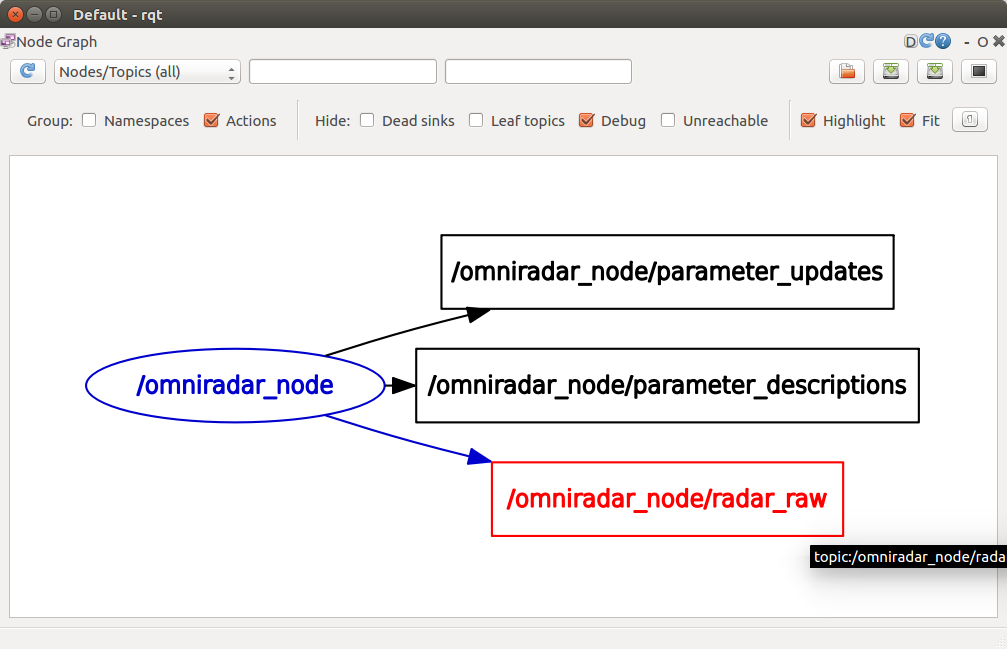
\includegraphics[width=0.5\textwidth]{https://rawgit.com/lalten/ma/master/screenshots/nodegraph.png}

While parameters from the ROS parameter server (as configured in the
launch) are respected, the node also offers a dynamic reconfigure server
to change RIC configuration string, number of sweeps and length of sweep
on the fly without the need to restart the node.
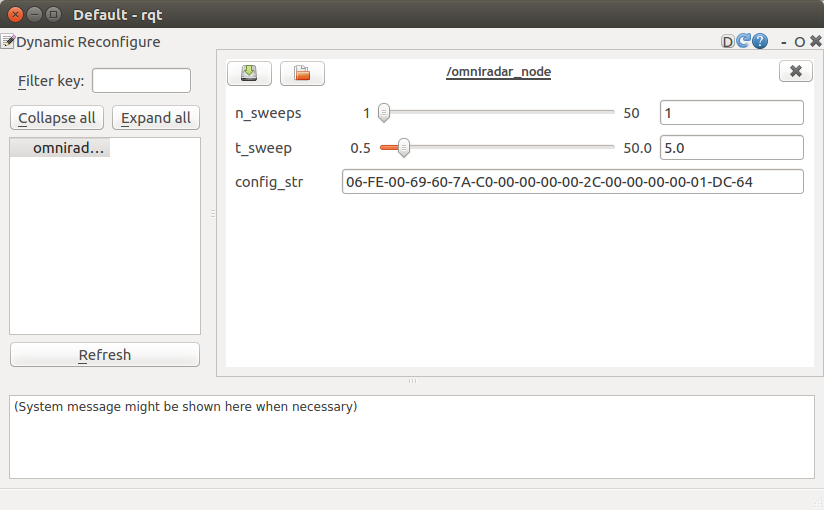
\includegraphics[width=0.5\textwidth]{https://rawgit.com/lalten/ma/master/screenshots/dynreconf.png}

The core of the node is a while loop that continuously triggers radar
echo acquisition and copies the result into a new
\texttt{omniradar::RadarEcho} message. The radar sensor update rate
could be increased by offloading the message assembly and data copying
into a C++11 lambda thread that is immediately detached.

\begin{Shaded}
\begin{Highlighting}[]
\BuiltInTok{std::}\NormalTok{lock_guard<}\BuiltInTok{std::}\NormalTok{mutex> lock_rdk(mtx_rdk);}
\KeywordTok{auto}\NormalTok{ t_echo = ros::Time::now();}
\KeywordTok{auto}\NormalTok{ p_echo = rdk->AcquireEcho(msg.n_sweeps);}

\BuiltInTok{std::}\NormalTok{thread t (}
\NormalTok{    [=] ()}
\NormalTok{    \{}
        \BuiltInTok{std::}\NormalTok{lock_guard<}\BuiltInTok{std::}\NormalTok{mutex> lock_msg(mtx_msg);}
\NormalTok{        msg.header.stamp = t_echo;}
\NormalTok{        msg.packed_echo.resize(p_echo->size());}
        \BuiltInTok{std::}\NormalTok{copy(p_echo->begin(), p_echo->end(), msg.packed_echo.begin());}
\NormalTok{        pub.publish(msg);}
\NormalTok{        msg.header.seq++;}
\NormalTok{    \}}
\NormalTok{);}
\NormalTok{t.detach();}
\end{Highlighting}
\end{Shaded}

The multithreading approach lets the node use between 100\% and 140\%
CPU (observed with \texttt{htop}).

\section{Matlab}\label{matlab}

Matlab (release R2017a) was chosen as implementation platform and
language because it allows quick prototyping, provides relatively easy
visualization, and, with the Robotics Toolbox, supports many ROS
features.

\subsection{Custom ROS message
support}\label{custom-ros-message-support}

It is necessary to install custom message support with the
\href{https://www.mathworks.com/help/robotics/ref/roboticsaddons.html}{roboticsAddon}
and
\href{https://www.mathworks.com/help/robotics/ug/create-custom-messages-from-ros-package.html}{generate}
the files to read in rosbags with \texttt{RadarEcho} type messages.

\section{Complementing sensors}\label{complementing-sensors}

TODO

\subsection{RGBD}\label{rgbd}

\subsection{Lidar}\label{lidar}

\section{Implementation}\label{implementation-1}

\subsection{Overview}\label{overview}

\subsection{Data path}\label{data-path}

\subsection{Code structure}\label{code-structure}

\subsection{Usage}\label{usage}

\begin{enumerate}
\def\labelenumi{\arabic{enumi}.}
\tightlist
\item
  Start robot, connect three sessions with \texttt{ssh\ zero2-pa}
\item
  Start ROS core with \texttt{roscore}
\item
  Start the node, with keyboard teleoperation and Cartographer Laser
  Slam:
  \texttt{roslaunch\ omniradar\ omniradar\_teleop\_lidarslam.launch}
\item
  Use \texttt{rqt} with the \emph{Dynamic Reconfigure} plugin to set the
  Omniradar node to generate the preferred number of sweeps and sweep
  duration. The configuration string can also be changed. The defaults
  are fine (One 5ms sweep)
\item
  \texttt{rosbag\ record\ /omniradar\_node/radar\_raw\ /odom\ /tf\ /map\ -O\ scan}
  will record a rosbag ``scan.bag'' containing all ROS messages with
  radar data, Kobuki odometry and slam map and transforms from
  Cartographer.
\item
  In the terminal running \texttt{roslaunch}, use the arrow keys to move
  the robot around (\(\uparrow\) and \(\downarrow\) to increase and
  decrease speed, \(\leftarrow\) and \(\rightarrow\) to increase and
  decrease rotation speed). \(E\) resets speed to zero and makes the
  robot halt.
\item
  After recording some interesting data, stop the rosbag record
  (\(Ctrl+C\)). Open a new terminal on your local machine and run
  \texttt{ssh\ zero2-pa\ "tar\ zcf\ -\ scan.bag"\ \textbar{}\ tar\ zxf\ -}.
  The rosbag will be transferred to your machine. Using ssh with the tar
  pipe is the fastest way to transfer the data (around \(100 Mbps\) on
  the BSH wifi). Compressing first (\texttt{rosbag\ compress\ scan.bag})
  and then sending takes a while on the not-so-powerful Odroid platform.
\item
  Optionally filter out unwanted transforms from the rosbag to speed up
  later processing:
  \texttt{rosbag\ filter\ scan.bag\ scan\_filtered.bag\ \textquotesingle{}(topic\ ==\ "/tf"\ and\ m.transforms{[}0{]}.child\_frame\_id\ ==\ "odom")\ or\ topic\ !=\ "/tf"\textquotesingle{}}
\item
  In Matlab, run
  \texttt{radar\_data\ =\ radar\_bag2array("/path/to/your/scan.bag");}.
  This will read the bag sequentially into memory and extract the data:
  The robot position is recorded from odometry information and corrected
  using the /map \(\rightarrow\) /odom transform as reported by slam
  localization. Cross range mileage is calculated as cumulative sum of
  distance between radar positions (as the radar is not mounted over the
  robot's rotation center, the radar mileage is different from robot
  mileage as soon as any rotational velocity is present). Lastly, all
  values are interpolated at the radar message timestamps. It is a good
  idea to save the function's output, using
  \texttt{save(\textquotesingle{}radar\_data/radar\_data\_scan.mat\textquotesingle{},\ \textquotesingle{}radar\_data\textquotesingle{})}
\item
  The radar data can now be analyzed. The
  \texttt{plot\_world\_projection} script can be used to get a good
  overview over raw data, doppler speeds, direction of arrival, and
  reprojection map.
\item
  To compare radar reprojection map and laser slam map, try the
  \texttt{test\_slam\_overlay} with the correct bag filename (the lidar
  map is extracted from that bag)
\end{enumerate}

\section{Data Preprocessing}\label{data-preprocessing}

TODO

\subsection{Rosbag to Matlab}\label{rosbag-to-matlab}

\subsection{(Odometry) Cross range
interpolation}\label{odometry-cross-range-interpolation}

\subsection{Raw Data Smoothing}\label{raw-data-smoothing}

After taking a single range reading, it will usually be relatively
noisy. One solution to getting cleaner range data with higher SNR is
oversampling. It is possible to use a moving average over a certain
accumulation distance to achieve this. However, the number of raw
samples is quite high and processing each sample takes a considerable
amount of time (some minutes for some minutes of recorded data). It is
better to make use of binning, with bins the width of the accumulation
distance. All samples in one bin are averaged to represent that bin's
value. This greatly improves processing time (to less than a second for
some minutes of recorded data).

Figure \#REF shows in gray the raw data of the first 20 range scan lines
from the ``Mancave'' dataset. It then compares different ways of
averaging over these 20 scans. All of them increase the SNR, because a
big part of the noise signal is statistically uncorrelated. Table \#REF
compares the RMS of the difference of each signal to the harmonic mean,
which gives the cleanest signal.

\begin{longtable}[]{@{}ll@{}}
\toprule
Signal & RMS of difference to harmonic mean\tabularnewline
\midrule
\endhead
Harmonic mean & 0\tabularnewline
Geometric mean & 0.144\tabularnewline
Arithmetic mean & 0.275\tabularnewline
50\%-Trim mean & 0.284\tabularnewline
Median & 0.318\tabularnewline
Raw & 1.064\tabularnewline
\bottomrule
\end{longtable}

The harmonic mean is defined as
\[harmmean(x_{1,2,...,n}) = \frac{n}{\frac1{x_1} + \frac1{x_2} + \cdots + \frac1{x_n}} = \frac{n}{\sum\limits_{i=1}^n \frac1{x_i}}\]
The geometric mean is defined as
\[geomean(x_{1,2,...,n}) = \left(\prod_{i=1}^n x_i \right)^\frac{1}{n} = \sqrt[n]{x_1 x_2 \cdots x_n}.\]
The arithmetic mean is defined as
\[mean(x_{1,2,...,n}) = \frac{1}{n}\sum_{i=1}^n x_i=\frac{x_1+x_2+\cdots+x_n}{n}\]
The 50\% trimmed mean is defined as the arithmetic mean of all except
the highest and lowest \(\frac{n}4\) data points, where \(n\) is the
number of data points. The median is defined as the value that lies
between the lower and the upper half of sample values.

\begin{figure}
\centering
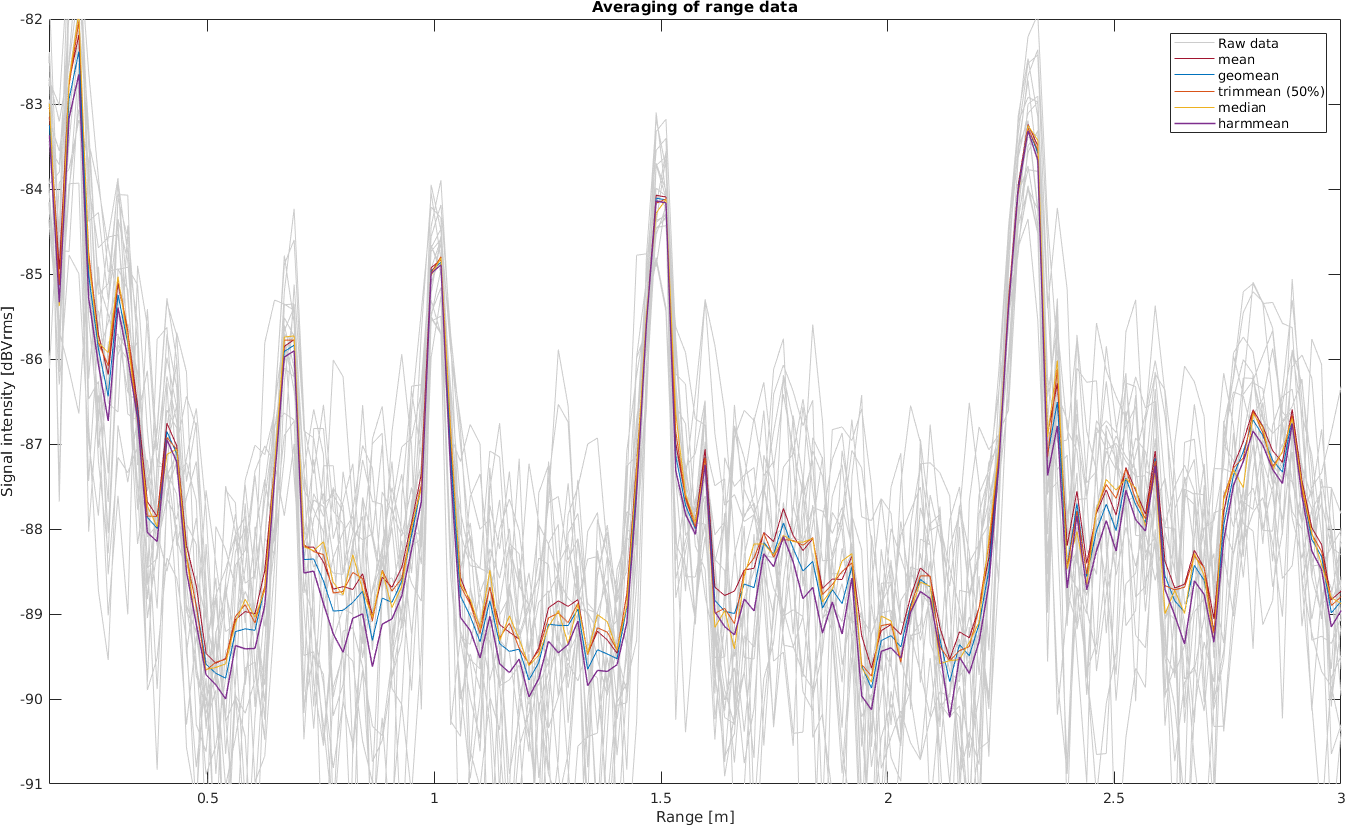
\includegraphics[width=0.5\textwidth]{https://rawgit.com/lalten/ma/master/figures/fig_compare_means.png}
\caption{restrict-height}
\end{figure}

Due to the good signal quality, the implementation uses the harmonic
mean to average the bins. Weighting the average with triangular or
Gauss-shaped weight distribution did not noticeably improve data quality
for any of the averaging methods.

Note that the range signal is not the only signal that needs to be
averaged in a range bin. All other parameters that are part of the range
scan need to be averaged as well. These parameters are mileage at scan
time, robot position and orientation, and robot speed. Sweep time and
down range bins don't change.

\section{Doppler Estimation with the Peak Gradient
Algorithm}\label{doppler-estimation-with-the-peak-gradient-algorithm}

The peak gradient algorithm is a way to find Doppler speeds from
consecutive range profiles.

\begin{figure}
\centering
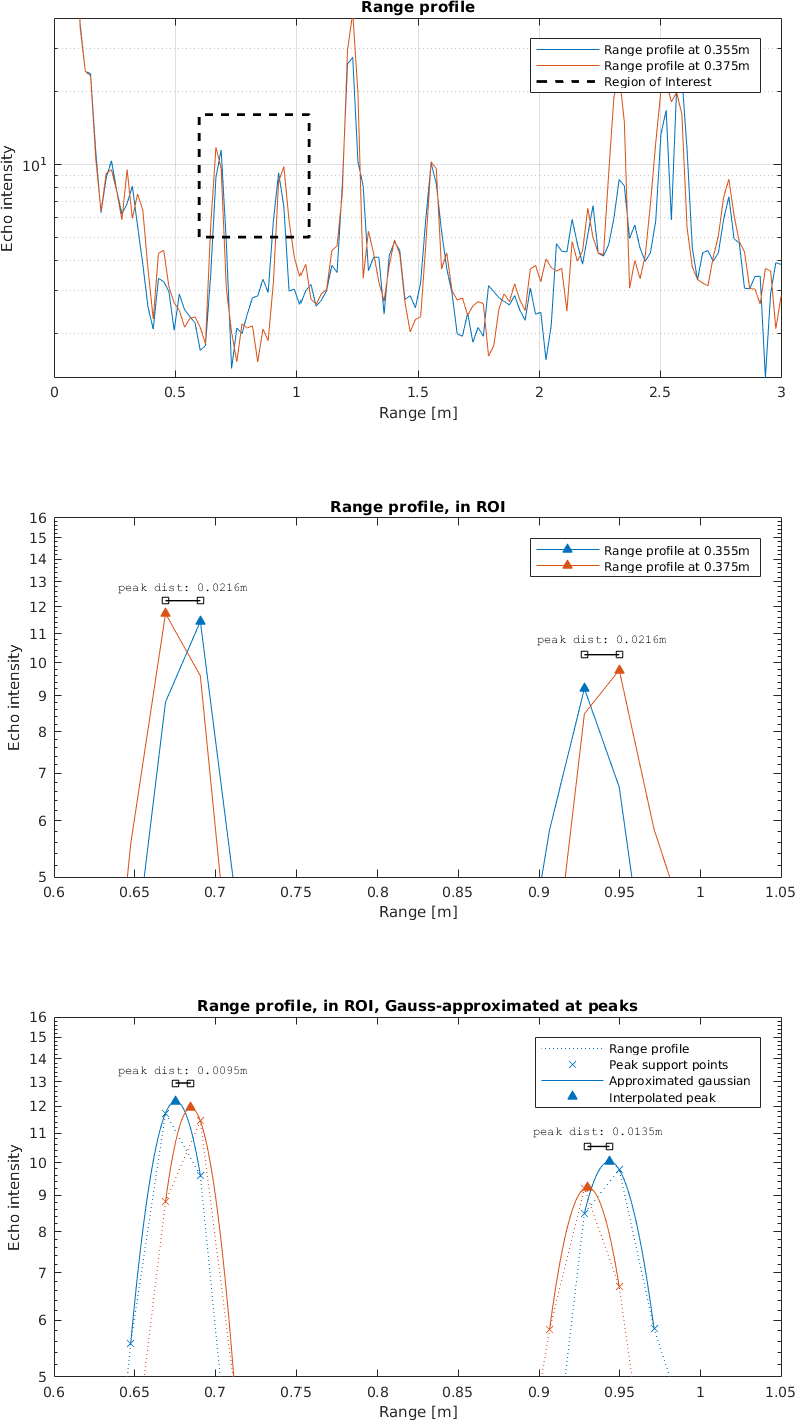
\includegraphics[width=0.5\textwidth]{https://rawgit.com/lalten/ma/master/figures/fig_explain_peak_gradient.png}
\caption{restrict-height}
\end{figure}

In figure \#REF the scans at radar mileage \(0.355m\) and \(0.375m\) of
a scene (``Basement'') are overlaid. Obviously the range profiles of the
two scans are very similar. However, as visible in figure \#REF some
peaks from target echoes are shifted, as the distance to the targets
changes with the radar moving through the scene. The rate at which the
distance to a target changes is its relative speed to the radar, the
Doppler speed.

Usually, speed is measured in distance per time. In this case, it
actually makes sense to ignore the scan's time stamps and look at the
cross range (driven mileage) instead. With the Doppler speed as change
of down range (distance to target) per cross range driven, calculations
become time independent and hence radar movement speed independent.

A target's distance from the radar is assumed to be at the range bin of
the corresponding peak in a scan's range profile. When a target's
distance changes the peak will shift, too. This is visible in figure
\#REF and we can read the Doppler speed from the figure. The peak around
\(0.67m\) moves \(d_{down,1} = 0.0216m\) closer in range, while the peak
around \(0.95m\) moves \(d_{down,2} = -0.0216m\) closer (i.e., away).
Combined with the change in cross range,
\(d_{cross} = 0.3752m - 0.3555m = 0.0197m\), we can calculate Doppler
speeds of \(v_{D,1} = \frac{d_{down,1}}{d_{cross}} = 109.55 \%\) (of
radar movement speed) and
\(v_{D,2} = \frac{d_{down,2}}{d_{cross}} = -109.55 \%\). If the speeds
were \(100\%\) and \(-100\%\) it would mean that the targets are directly
ahead and directly behind the moving radar. Speeds over 100\% are
however impossible in a static environment where all relative target
motion is caused by the radar movement. The targets are therefore either
dynamic and moving by themselves, or the peak locations that determined
those too-high speeds were not exact. Since we know that there were no
dynamic moving objects in the controlled environment of the scan, the
latter must be the case.

This effect of imprecise target peak localization and Doppler speed
estimation could be overcome by averaging noisy data so that the average
peak distance is close to the actual change in target range. A lot more
scans are necessary for that though, and scan oversampling needs to be
drastically reduced. This would lead to lower SNR, which means that some
peaks with lower echo intensity could not be detected.

With higher downrange resolution, peaks could be localized more
precisely. However, the down range resolution is limited by the
available bandwidth of the radar sensor. In the Omniradar RIC60A, up to
7GHz are available, which is already extremely high. Its range
resolution \(dR\) is \(\frac{c}{2 BW}\), which is roughly \(2.1cm\). With
this method, \(dR\) is of course the smallest measurable change of
target range.

The localization of peaks is however not limited by range resolution,
but by range accuracy, which mainly depends on SNR. It is much better
than range resolution with \(\sigma_R = \frac{dR}{\sqrt{SNR}}\). This
can be utilized with subsample peak interpolation.

\subsection{Inter-scan vs Intra-scan Doppler
estimation}\label{inter-scan-vs-intra-scan-doppler-estimation}

For correct Doppler estimation it is important to have the exact timing,
or for relative Doppler speed, exact cross range mileage of the range
scans whose peaks are compared in the peak gradient algorithm.

The Omniradar sensor can send multiple consecutive sweeps without any
delay between them. The timing will then be very exact, because the
precise length of one sweep is known. However, the number of sweeps in
such a set of sweeps is limited (transmission of high data volumes will
often fail), so they can't be average to be smoothed through
oversampling and will be noisy. Smaller peaks will then not be detected
reliably. Another problem with this approach is that it will give target
Doppler speeds in change of down range over time, but not the robot
speed-invariant relative Doppler speed in change of down range over
change of cross range.

Inter-scan comparison gives better Doppler estimation, because the data
can be smoothed through oversampling first. Consecutive sweeps can still
be used: They need to be separated into individual scans with timestamps
adjusted to \(t_{msg} + i\cdot t_{sweep}\) (with message timestamp
\(t_{msg}\), consecutive sweep index \(i\) and sweep duration
\(t_{sweep}\)) and cross range mileage interpolated at that timestamp.

\subsection{Subsample peak
interpolation}\label{subsample-peak-interpolation}

In subsample peak interpolation a curve is fitted on several supporting
points in the coarse-resolution data. In the case of a single,
non-overlapping radar echo peak, a Gaussian pulse of the form
\[g_i(x) = a_i e^{-b_i ( x - c_i )^2}\] is a good approximation. In
figure \#REF, the data point of the respective peak as well as its left
and right neighbors are fitted with a Gaussian. The fit parameters
\(a\), \(b\) and \(c\) are calculated using
\href{https://www.mathworks.com/matlabcentral/fileexchange/24465}{Travis
Wiens's crit\_interp\_g} function.

As evident by visual inspection, the intensity and location of the
fitted function's maximum are much closer to the real value.

With the same procedure as explained above, we measure peak distance
shifts of \(d_{down,1}=9.510mm\) and \(d_{down,2}=-13.52mm\) in figure
\#REF and can hence estimate Doppler speeds of \(v_{D,1}=48.26\%\) and
\(v_{D,2}=-68.63\%\) of radar movement speed. These values are a much
more plausible estimation and generally work very well when used to
calculate the reprojection angle in the reprojection method.

\subsection{Peak matching}\label{peak-matching}

Visually it seems clear which peaks belong to each other in consecutive
range scan lines. But for the algorithm this poses a challenge. Range
scan lines usually don't have the same number of peaks because new
targets can appear, old targets can disappear, noise can temporarily
mask out targets peaks and target arcs cross each other. However if the
cross range difference, i.e.~the driven distance between scans, is not
too high, a single target will not change very much in both range and
echo intensity. This allows the detection of peak matches, between which
the Doppler speed will be calculated. The parameters for peak matching
tolerance are therefor allowed intensity change
\[max. ValueSearchArea = \delta \frac{I}{\Delta d_{cross}}\] with
intensity change factor \(\delta I\) and cross range difference
\(\Delta d_{cross}\) allowed range change
\[max. LocSearchArea = \frac{\Delta d_{down}{\Delta d_{cross}}} = v_D = \alpha~v_R\]
which is more easily expressed as maximum Doppler speed \(v_D\) in
percent of robot speed \(v_R\). Good values are a factor of
\(5 cm^{-1}\) as maximum intensity change factor and a factor of
\(2 v_R\) as maximum Doppler speed.

\subsubsection{Minimum Peak height}\label{minimum-peak-height}

\subsection{Transmit crosstalk
suppression}\label{transmit-crosstalk-suppression}

At low range, spurious peaks occur. The first one is caused by transmit
antenna crosstalk and is visible as very high intensity echo around
\(d_{down}=0\). After the transmit antenna crosstalk spike there is
another peak around \(d_{down}=0.25m\) which is consistently visible. It
can be explained with static objects sitting close to the radar,
i.e.~robot parts and the floor below the robot.

These spurious peaks create two problems: (1) automatic color scaling or
height scaling respectively in plots is more difficult, and (2) high
intensity false positives would be visible next to the robot path in the
final map.

Hence these spurious peaks must be ignored during peak detection. This
can be achieved in two ways. The first is to simply replace all data
values under a down range limit \(d_{mute}\) (usually
\(d_{mute}=0.30m\)) with \(NaN\) values. For the second way, one effect
of range compensation is exploited. As shown in figure \#REF, the spike
that previously had its maximum in the first range bin, at
\(d_{down}=0\), now has its maximum in a later range bin. The reason is
that the range compensation factor at \(d_{down}=0\) is \(r(0) = 0\) but
\(r(d_{down}>0) > 0\). As the transmit peak now has a maximum with
neighbors lower than its maximum, \texttt{findpeaks} can find it. Color
scaling can then be made to work correctly by clipping all values higher
than the \emph{second highest} peak. The Peak Gradient Algorithm also
has an optional parameter \texttt{SkipFirstPeak} which, when set to
\(true\), ignores the first peak in each range scan line. This can help
to ignore these echoes.

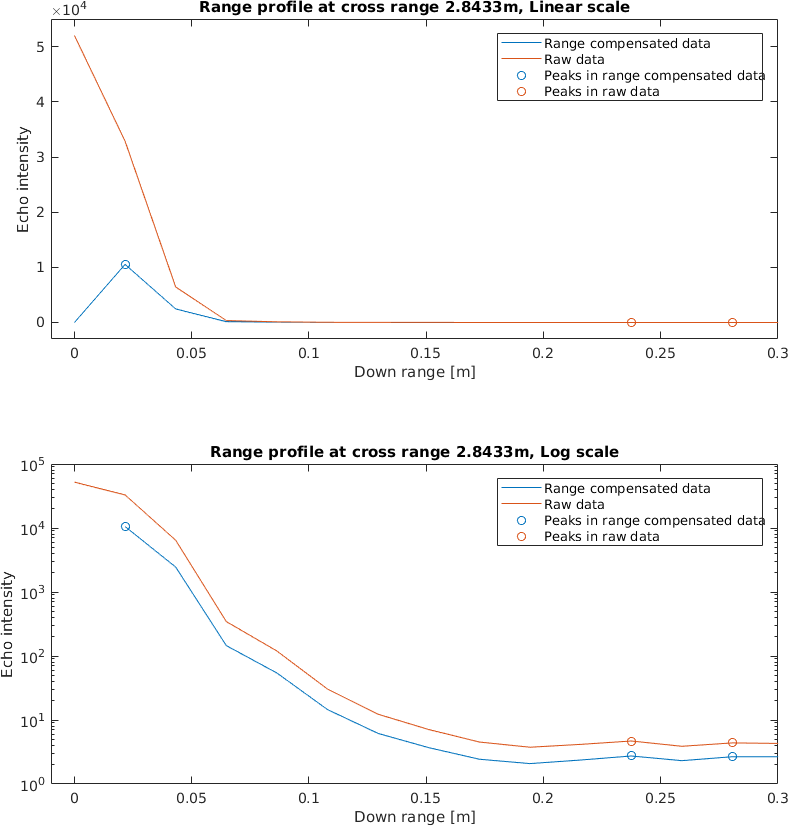
\includegraphics[width=0.5\textwidth]{https://rawgit.com/lalten/ma/master/figures/fig_range_compensation_transmit_spike.png}
Note that the \(0\) value at \(d_{down}=0\) won't be displayed in log
scale.

\subsection{Peaks overlaps at crossing target
arcs}\label{peaks-overlaps-at-crossing-target-arcs}

\subsection{Output}\label{output}

\subsection{Limitations}\label{limitations-1}

\subsubsection{Problems with imperfect fit function for
subsampling}\label{problems-with-imperfect-fit-function-for-subsampling}

\subsubsection{Problems with close
targets}\label{problems-with-close-targets}

When Doppler speed is measured directly using FMCW, there will be
several Doppler peaks, each representing a different target at the same
range but with individual relative speeds. With the Peak Gradient
Algorithm however, multiple targets at the same range are difficult to
separate. In some cases this is only a temporary problem and is resolved
by the radar moving a little farther so the ranges are separated by more
than the range resolution. Sometimes however some peaks come from
point-like targets that are close together, like a parts of a wall. This
bundle of targets is however not always separated by the same range.
Especially in the case of a wall, the traces of visible points will
cross each other as they slide on the sine arc (see figure). When the
points are close together, only the brightest spots will be seen as
peaks, and the trace of the detected peak matches will describe a
squiggly motion. This causes the estimated Doppler speed to wander
around the common speed. To combat this effect, a higher accumulation
distance can be used during oversampling preprocessing, so the peaks
move together so closely that they actually form a single target.

\begin{figure}
\centering
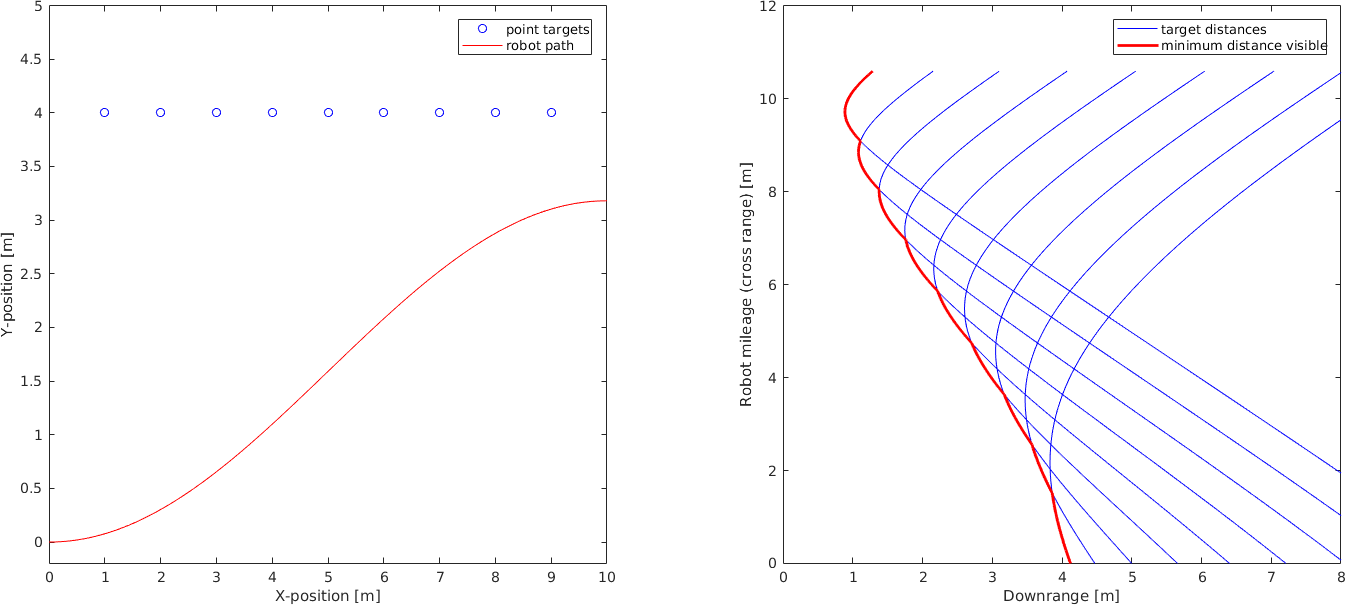
\includegraphics[width=0.5\textwidth]{https://rawgit.com/lalten/ma/master/figures/fig_squiggly_doppler_at_wall.png}
\caption{restrict-height}
\end{figure}

\section{DOA Implementation}\label{doa-implementation}

As described in \#REF, the Direction of Arrival (DOA) angle can be
measured from the phase difference at the receiving antennas of a
multistatic radar.

In the case of RIC60A the antenna separation \(d\) is \(1.16mm\) and
wavelength \(\lambda\) is \(\lambda=\frac{c}{60GHz}=5.0mm\) (with speed
of light \(c\)).

Figures \#REF and \#REF show the range profile and phase shift of the
``Basement'' scan. The phase shift is very noisy in the regions without
a target peak in the range profile but exhibits steady values following
a gradient over targets.

\begin{figure}
\centering
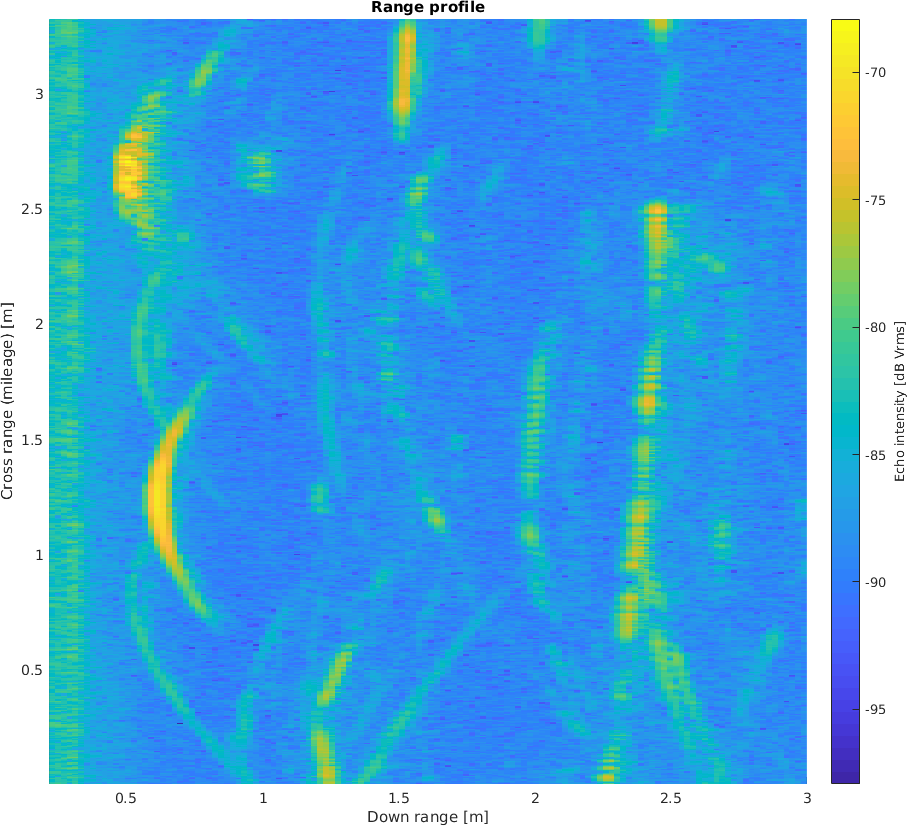
\includegraphics[width=0.5\textwidth]{https://rawgit.com/lalten/ma/master/figures/fig_range.png}
\caption{restrict-height}
\end{figure}

\begin{figure}
\centering
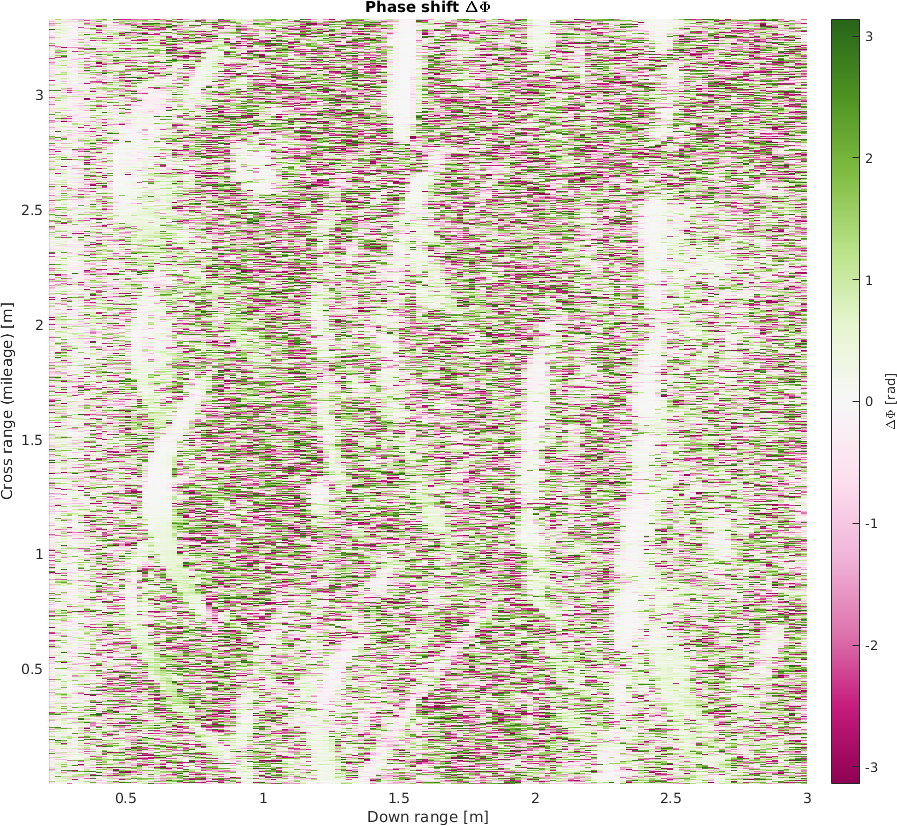
\includegraphics[width=0.5\textwidth]{https://rawgit.com/lalten/ma/master/figures/fig_phase_shift.png}
\caption{restrict-height}
\end{figure}

Four steps are performed to get a reasonable estimation of direction of
arrival. \textbf{Peak detection}. In a first step, target peaks in the
range profile are detected. The algorithm records for each peak in each
range scan line its fitted interpolated location, full width at half
maximum, and matching peaks in adjacent lines regarding value and
location. \textbf{Down range averaging}. In each range scan and at every
detected target peak, the phase shift is averaged over the width of the
respective detected peak. The average is weighted using the Gaussian fit
from subsample peak interpolation. \textbf{Cross range averaging}. In
every range scan line, each peaks phase shift is averaged over a
configurable accumulation distance in cross range dimension. This is
done by taking the arithmetic mean of all the phase shifts at all
matching peaks (regarding value and down range location) within
accumulation distance in cross range dimension. \textbf{Cut out}. Noisy
values at non-target peak range bins are masked out. \textbf{DOA
calculation}. In each scan line, each peaks direction of arrival
\(\theta\) is calculated from the smoothed phase shift values, using
formula \#REF.

Figure \#REF shows the result of these four steps applied on the data of
the ``Basement'' scan. The direction of arrival seems plausible: In this
side-facing scan the robot passed some metal cans. Apparently the radar
sensor was not mounted perfectly orthogonal to the robot's movement
direction (which is not necessary for the reprojection method), but was
slightly off by. This can be seen at the closest points of the target
arcs. At the pericenter the line of sight to a target is orthogonal to
the robot's movement direction, but the DOA value shows to be around 5
to 10 degrees.

\begin{figure}
\centering
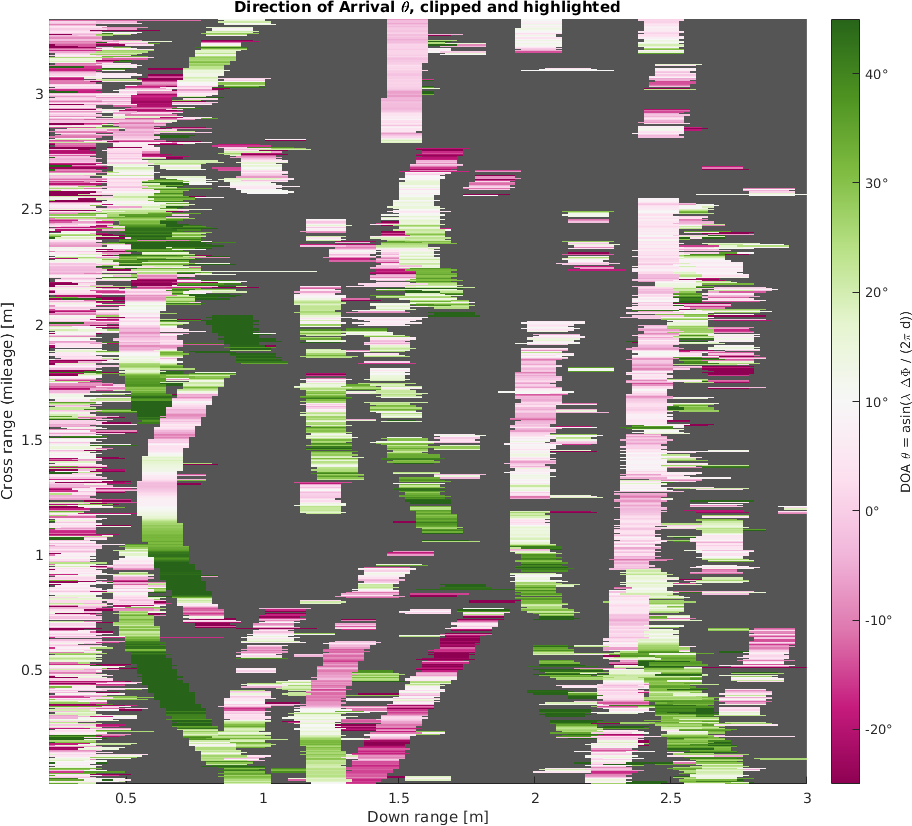
\includegraphics[width=0.5\textwidth]{https://rawgit.com/lalten/ma/master/figures/fig_doa.png}
\caption{restrict-height}
\end{figure}

Note that if the radar sensor is mounted inverted (rotated by 180°), DOA
values have to be multiplied by \(-1\) to keep right and left where they
are.

\section{Reprojection Mapping}\label{reprojection-mapping}

\subsection{Orientation parameters}\label{orientation-parameters}

Before the reprojection can be executed, the physical orientation of the
radar sensor needs to be known to the algorithm. In the implementation,
the two boolean parameters \texttt{forward\_looking} and
\texttt{mount\_inverted} control the behaviour. If the radar's squint
angle and angle sensitivity are such that the field of view reaches both
sides of the robot path, the \texttt{forward\_looking} parameter needs
to be enabled. This enables the processing of DOA data to find the sign
of every target's reprojection angle i.e.~if it is to the left or right
side of the robot's motion path. If the radar is mounted in an
upside-down configuration the squint angle is not affected, but if the
DOA values are processed they need to be mirrored (multiplication with
\(-1\)) because the left and right antennas are switched. Otherwise,
targets will be projected to the wrong side of the robot's path.

\subsection{Projection direction}\label{projection-direction}

The radar reprojection can be executed as forward or backward mapping.
The proof of concept implementation has an optional parameter
\texttt{ProjectionMethod} to switch between forward and backward
mapping.

\subsubsection{Backward mapping}\label{backward-mapping}

If backward mapping is enabled, the reprojection algorithm still
operates range scan line based, but iterates over each pixel in the map.
While this is computationally much more intensive, it allows to add
negative information by reducing the map's value at pixels that are
known to not contain a target because the range scan line does not
feature a peak at that range.

\begin{verbatim}
foreach range_scan_line in range_scan_lines
  foreach pixel in map
    pixel_angle = robot.get_angle_to(pixel)
    distance = robot.get_distance_to(pixel)
    if distance < max_range && pixel_angle in field_of_view_range
      range_bin = range_scan_line.interpolate_at(distance)
      if range_bin.has_peak
        peak_angle = range_bin.peak.doppler.to_angle
        if peak_angle == pixel_angle
          map.at(pixel).add(range_bin.value)
      else
        map.at(pixel).reduce_value
\end{verbatim}

\subsubsection{Forward mapping}\label{forward-mapping}

In forward mapping, the reprojection algorithm iterates over each range
bin in each range scan line. Detected peaks are cut out and reprojected
to a position on the map which is calculated from relative Doppler
speed, range, and robot position. The projection target coordinates
don't usually fall exactly on the map grid points. The implementation
uses sample splitting to distribute a value over the nearest pixels in
this case.

\begin{verbatim}
foreach range_scan_line in range_scan_lines
  foreach peak in range_scan_line
    foreach range_bin in peak
      target_coords = get_coords(robot.position, range_bin.range, peak.doppler)
      weights, neighborhood = split_sample(target_coords)
      map.at(neighborhood).add(weights, range_bin.value)
\end{verbatim}

\subsection{Sample splitting}\label{sample-splitting}

To avoid aliasing when projecting a pixel in the forward projection
direction, the sample is split over the four closest map pixels. The
split is weighted with the distance of the target coordinates to the
closest pixel centers.

If the target coordinate is \(p_{target}=(x_t, y_t)\), then the
horizontal and vertical distributions \(\nu_h\) and \(\nu_v\),
respectively, are \[
\nu_h = \frac{x_t - \lfloor x_t \rfloor}{\lceil x_t \rceil - \lfloor x_t \rfloor} \\
\nu_v = \frac{y_t - \lfloor y_t \rfloor}{\lceil y_t \rceil - \lfloor y_t \rfloor}
\]

The pixel weights \(p_{x,y}\) are then \[
p_{\lfloor x_t \rfloor, \lfloor y_t \rfloor} = \nu_v \nu_h\\
p_{\lfloor x_t \rfloor, \lceil y_t \rceil} = \nu_v (1 - \nu_h)\\
p_{\lceil x_t \rceil, \lfloor y_t \rfloor} =  (1 - \nu_v) \nu_h\\
p_{\lceil x_t \rceil, \lceil y_t \rceil} = (1 - \nu_v) (1 - \nu_h)
\] , such that \[
\sum\limits_{
x \in \{\lceil x_t \rceil, \lfloor x_t \rfloor\}\\
y \in \{\lceil y_t \rceil, \lfloor y_t \rfloor\}
} p_{x,y} = 1
\]

In the special case where $y\_t = \lceil y\_t \rceil = \lfloor y\_t\rfloor$ there are only two instead of the four neighboring pixels. Their weights \(p_{x,y}\) are \[
p_{\lfloor x_t \rfloor, y_t} = \nu_h\\
p_{\lceil x_t \rceil, y_t} = (1 - \nu_h)
\] The same applies when $x\_t = \lceil x\_t \rceil = \lfloor x\_t\rfloor$: \[
p_{x_t, \lfloor y_t \rfloor} = \nu_v\\
p_{x_t, \lceil y_t \rceil} = (1 - \nu_v)
\] And lastly, if
(\(y_t = \lceil y_t \rceil = \lfloor y_t \rfloor ) \land (x_t = \lceil x_t \rceil = \lfloor x_t \rfloor )\),
then \(p_{x_t, y_t} = 1\)

\begin{figure}
\centering
\includegraphics[width=0.5\textwidth]{"https://rawgit.com/lalten/ma/master/diagrams/Sample splitting"}
\caption{restrict-height}
\end{figure}

\subsection{Range compensation}\label{range-compensation}

As evident from the radar equation \#REF, echo intensity decreases with
the fourth power of distance. This has the effect that reprojected
targets appear brighter when they are mapped from close distance; but
most importantly, when targets are detected from a far distance, mapped
intensities are decreased due to the map's averaging.

This attenuation can be compensated with a range-based compensation
factor \(f_r\) with \[f_r(d_{down}) = {
\left(
c_a + (
\frac{{d_{down}}{c_b}}
+ c_c)^{-4}
\right) ^ {-1}
}\]



Figure \#REF shows the range profile of the ``Torture Chamber'' scan
both as oversampled raw values (top subplot) and with range compensation
enabled (bottom subplot). The middle subplot details the range scan line
at one cross range highlighted by the red lines. Inspecting this detail
graph reveals that both target peaks and noise floor are lowered in the
near range, while the noise floor stays constant in the far range. This
helps to keep a target's intensity at at least similar values over all
ranges in the map.

\begin{figure}
\centering
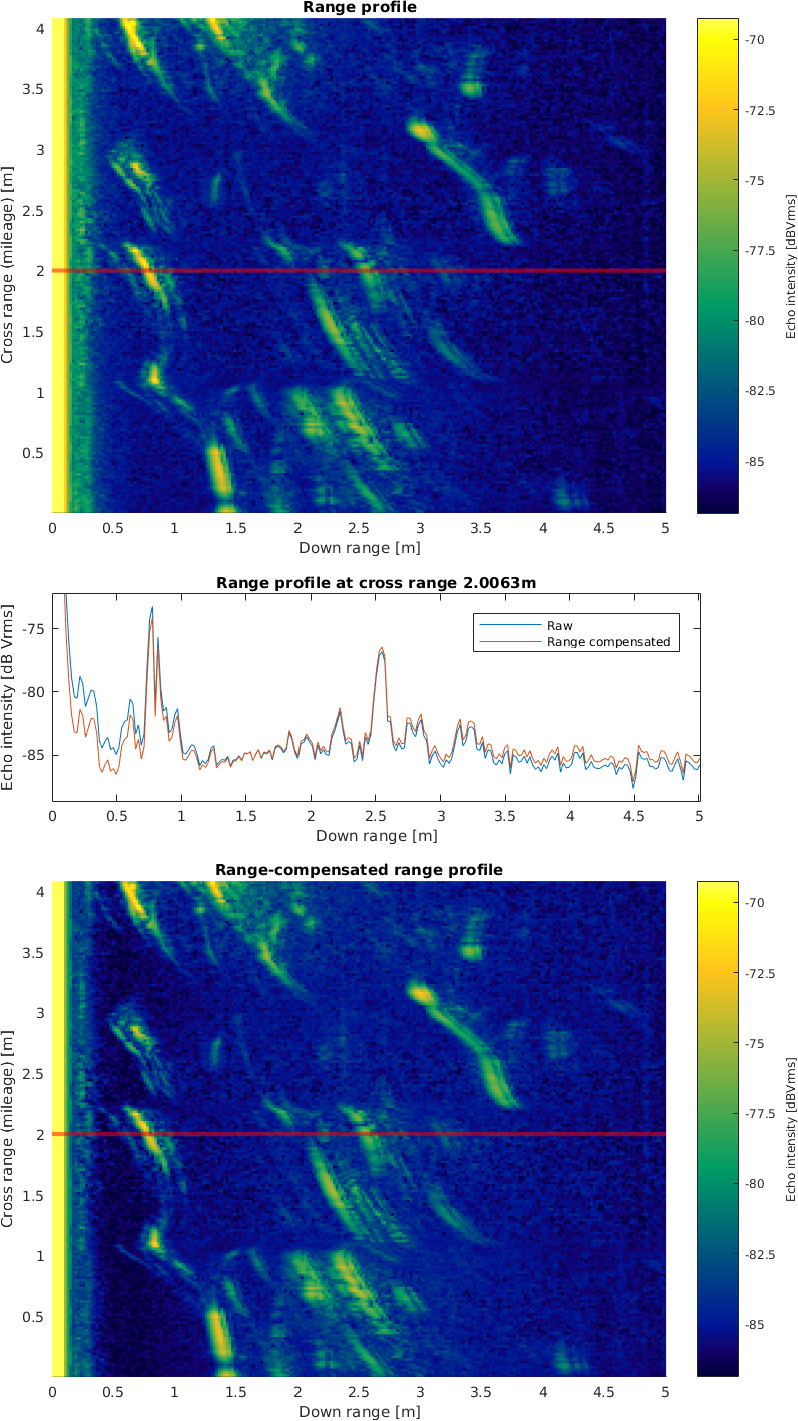
\includegraphics[width=0.5\textwidth]{https://rawgit.com/lalten/ma/master/figures/fig_range_compensation.png}
\caption{restrict-height}
\end{figure}

\subsection{Angle sensitivity
compensation}\label{angle-sensitivity-compensation}

The intensity of a target peak depends on its angle with respect to the
antenna. The angle is unknown before the Doppler speed is estimated, so
the knowledge about echo attenuation caused by antenna angle sensitivity
can not be used to improve peak detection. But the echo intensity
influences how a target is represented on the reprojection map. Since
the map averages all reprojections to any given point a low intensity
echo will reduce the visibility of a target on the map. This can however
be compensated by multiplying detected target peak heights with a factor
that is based on the angle the target is believed to be seen under.

The angle compensation factor curve was found by experiment. A strong
point target (a retroreflector) was placed at a known range away from
the robot. The robot was then made to rotate around itself, such that
the target comes into view and leaves again. Meanwhile, the radar scans,
together with robot odometry were recorded.

The radar was not mounted over the center of rotation of the robot. This
way, the radar did describe a circular path whose mileage can be
calculated. The angle compensation measurement can hence be visualized
in figure \#REF in the usual range profile with echo intensities over
cross versus down range. The range of the retroreflector varies with
twice the distance of the radar to the robot's rotation center, but only
the orientation is interesting - the range can just be summed up over
the range bins the target is visible in (in this case,
\(0.45m - 0.85m\)).

In figure \#REF, the same range scan lines are sorted by robot
orientation during the scan. After the explained summing in down range
dimension the intensity (absolute value of complex signal) data of both
antennas is binned separately over 60 orientations from \(-\pi\) to
\(\pi\).

The manufacturer later provided angle sensitivity measurements of the
IC's batch (see figure \#REF). The measurements show that the
experimental approach produced valid results.

The compensation factor \(f_a\) for each angle is finally composed using
the formula

\[m = \max \left( \max (s_{Rx1}), \max (s_{Rx2}) \right)\] \[
f_a = \frac{1}{2}
  \left(
    \frac{m}{ s_{Rx1} } +
    \frac{m}{ s_{Rx2} }
  \right)
\]

Multiplicating a peak which is to be reprojected at angle \(\alpha\)
with angle compensation factor \(f_a(\alpha)\) results in a peak height
that is independent of observation angle.

\begin{figure}
\centering
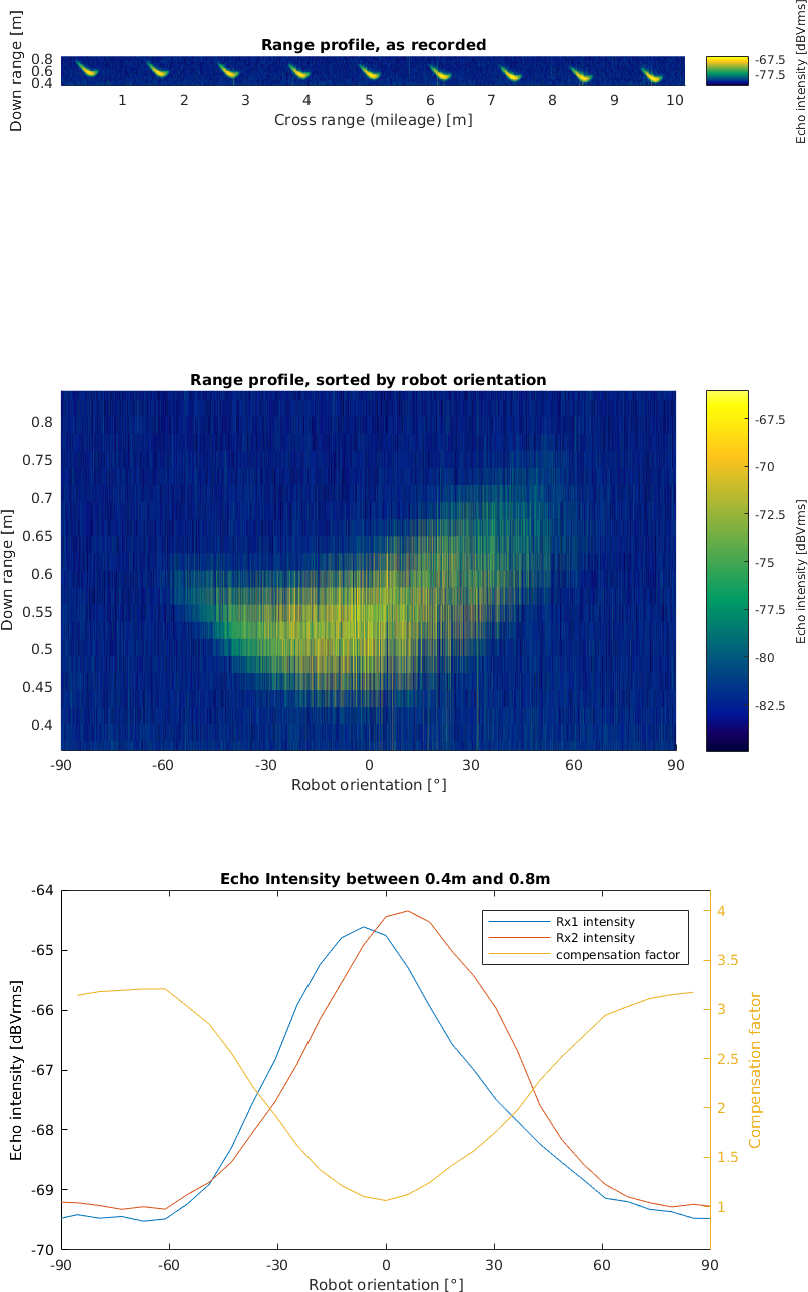
\includegraphics[width=0.5\textwidth]{https://rawgit.com/lalten/ma/master/figures/fig_angle_compensation.png}
\caption{restrict-height}
\end{figure}

\subsection{Angle compensation
window}\label{angle-compensation-window}

Detected peaks are not in a single range bin, but form a curve over
several range bins. Multiplicating each of these range bin's values with
the same \(f_a\) does work, but leaves hard edges. It is better to
multiplicate the peak with a window function with height \(f_a\). The
implementation the window \(w\): \[
w(x,f_a) = 1 + (f_a - 1)
~e ^ {
 -\frac{ \left( {x - p_x} \right) ^ 2 }
       {p_w}
}
\] where \(p_x\) is the peaks subsample-interpolated peak location in
down range space and
$$
p_w = \cfrac{
\left( \frac{fwhm}{4}  \right) ^2
}{
4 ln(2)}
$$ is
the peaks width, where \(fwhm\) is the full width at half maximum as
found by the subsample-interpolated peak fit.

Figure \#REF show a glass wall in the ``Racetrack'' scan. In the top
subplot, only range compensation is applied. In the middle subplot,
angle compensation is switched on. In the bottom subplot, both angle
compensation and angle compensation windowing are switched on. The
figure shows how angle compensation helps to keep the echo intensity of
a mapped object at the same level, regardless of the angle at which it
is seen by the radar.

\begin{figure}
\centering
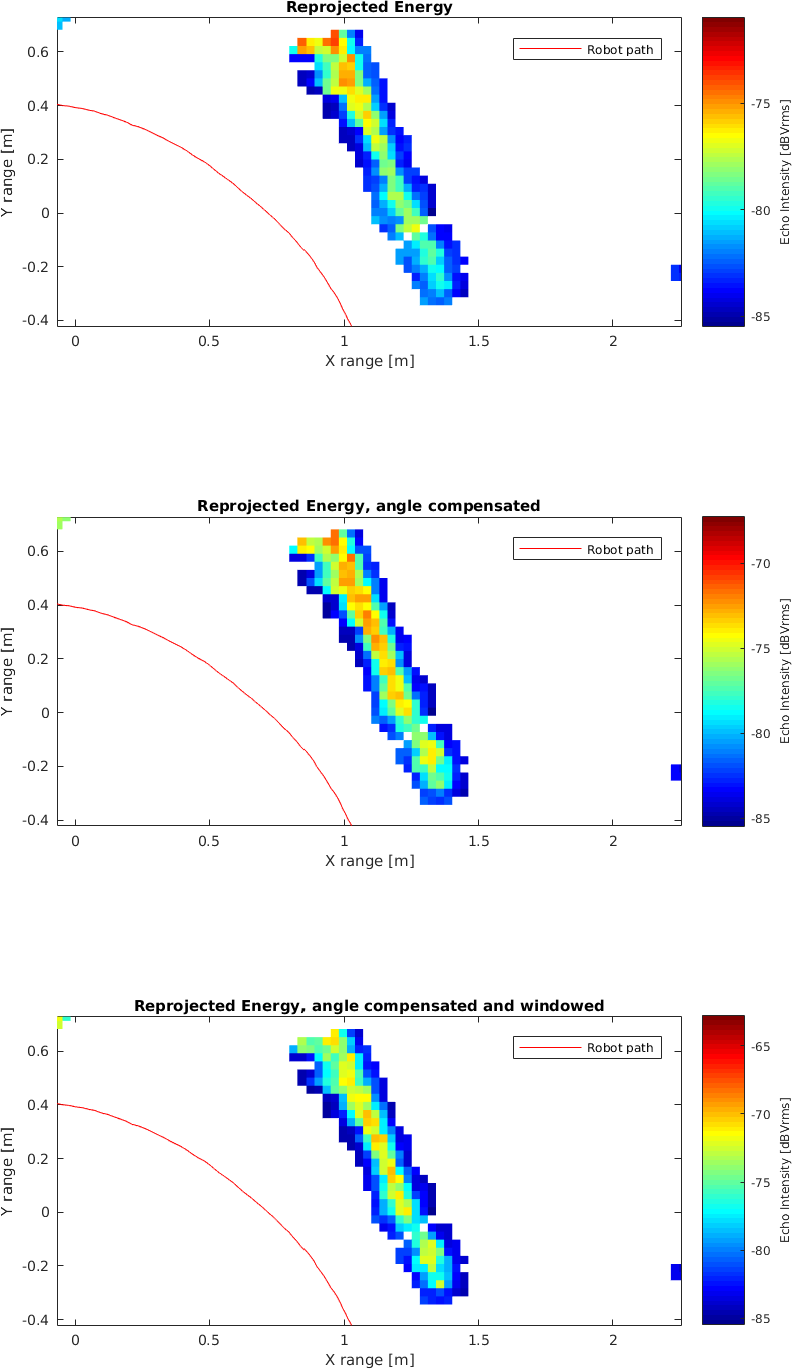
\includegraphics[width=0.5\textwidth]{https://rawgit.com/lalten/ma/master/figures/fig_angle_compensation_comparison.png}
\caption{restrict-height}
\end{figure}

\subsection{World map resolution}\label{world-map-resolution}
